\chapter{Results and Performance Analysis}
    In this chapter we are going to show the results of our research work along with an analysis of how performance our proposed model outputs. Here, we have showed the results and analysis with respect to several metrics and visualizations.
    
    We have trained our model for more than 100000 steps with a batch size of 24. Here, we are showing results by several parameters in different metrics.
    
    \section{Precision at Different Training Steps}
        During the training process running we have triggered evaluation of the model on the validation data at different checkpoints. These checkpoints are stored against the number of steps the training process completed.
        We show the graphs of the number of Training Steps versus Different Average Precision for different metrics which illustrates the changing history of the model's performance throughout the training process.
        
        \subsection{Average Precision for Different IoU Thresholds}
            Here, we show the model's performance taking the Average Precision considering different minimum \acrfull{iou} thresholds as the threshold for True Positive detection.
                        
            \begin{figure}
                \centering
                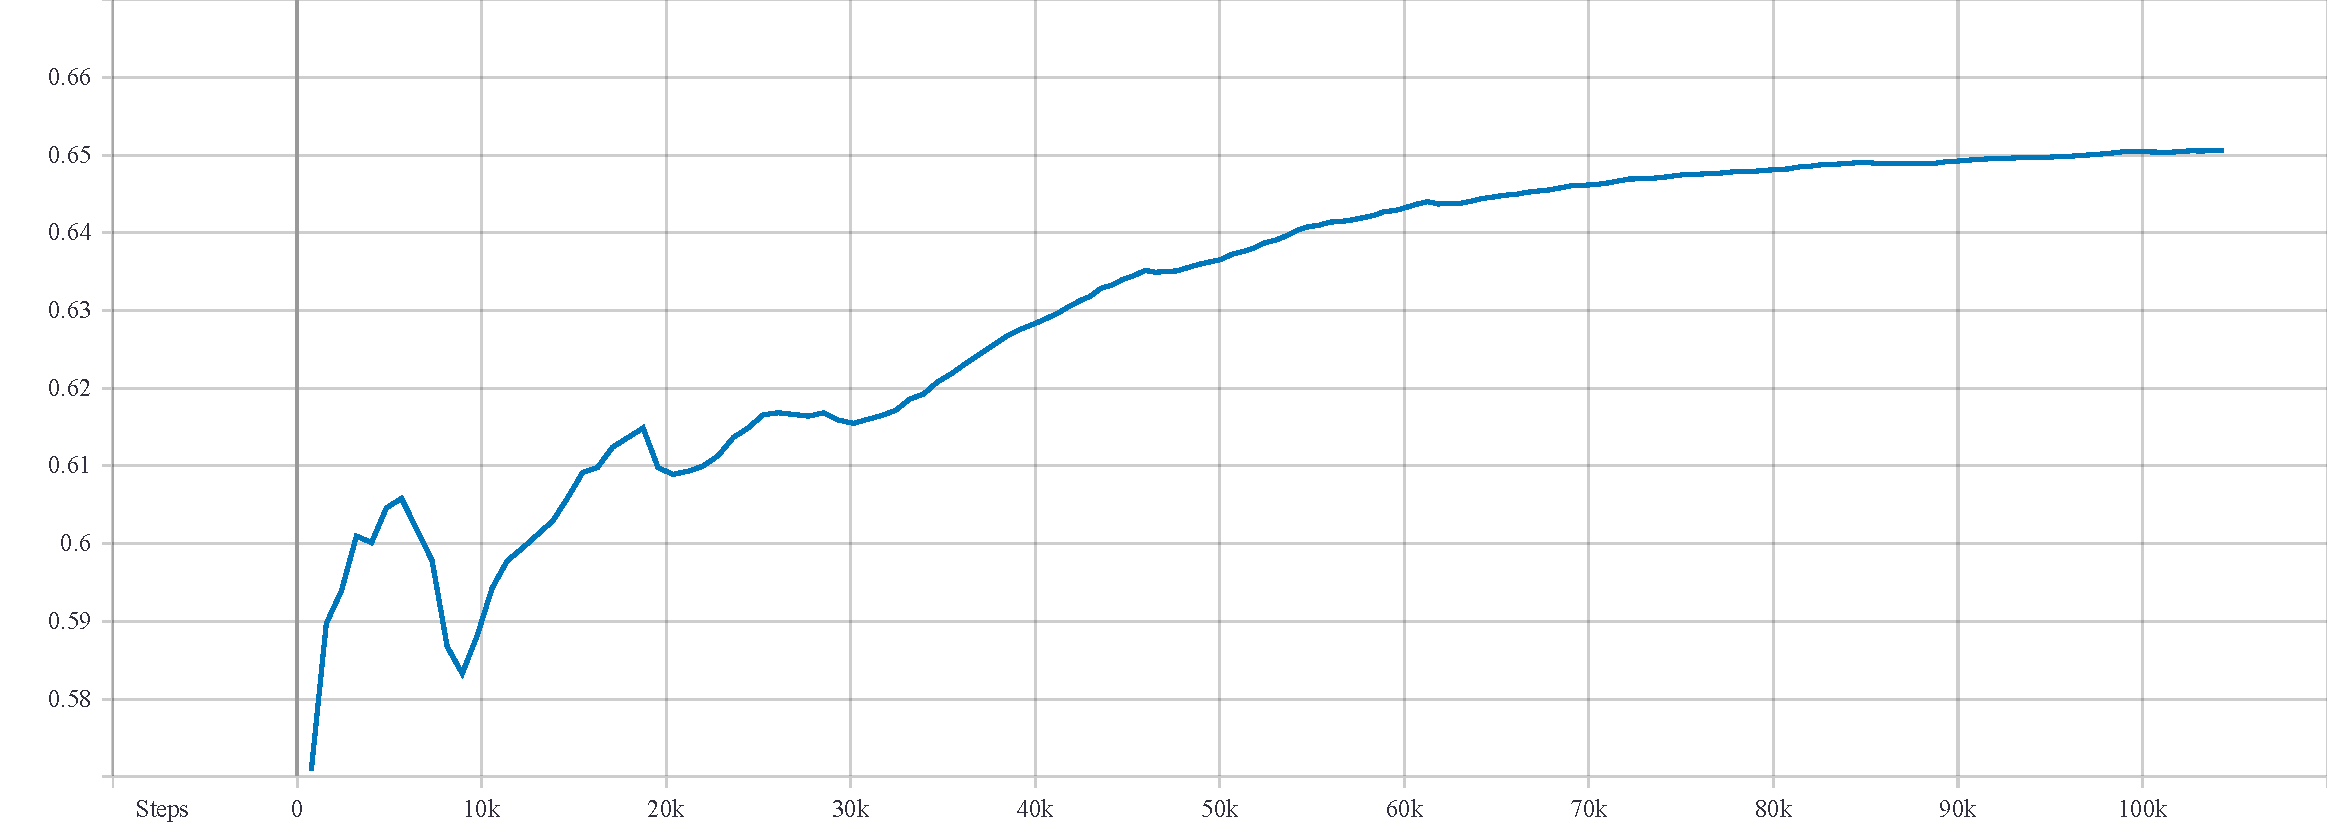
\includegraphics[width=\textwidth]{mAP-50-IoU}
                \caption{Changes of Precision at Different Training Steps for 50\% IoU}
                \label{fig:precision_iou50}
            \end{figure}
            
            \begin{figure}
                \centering
                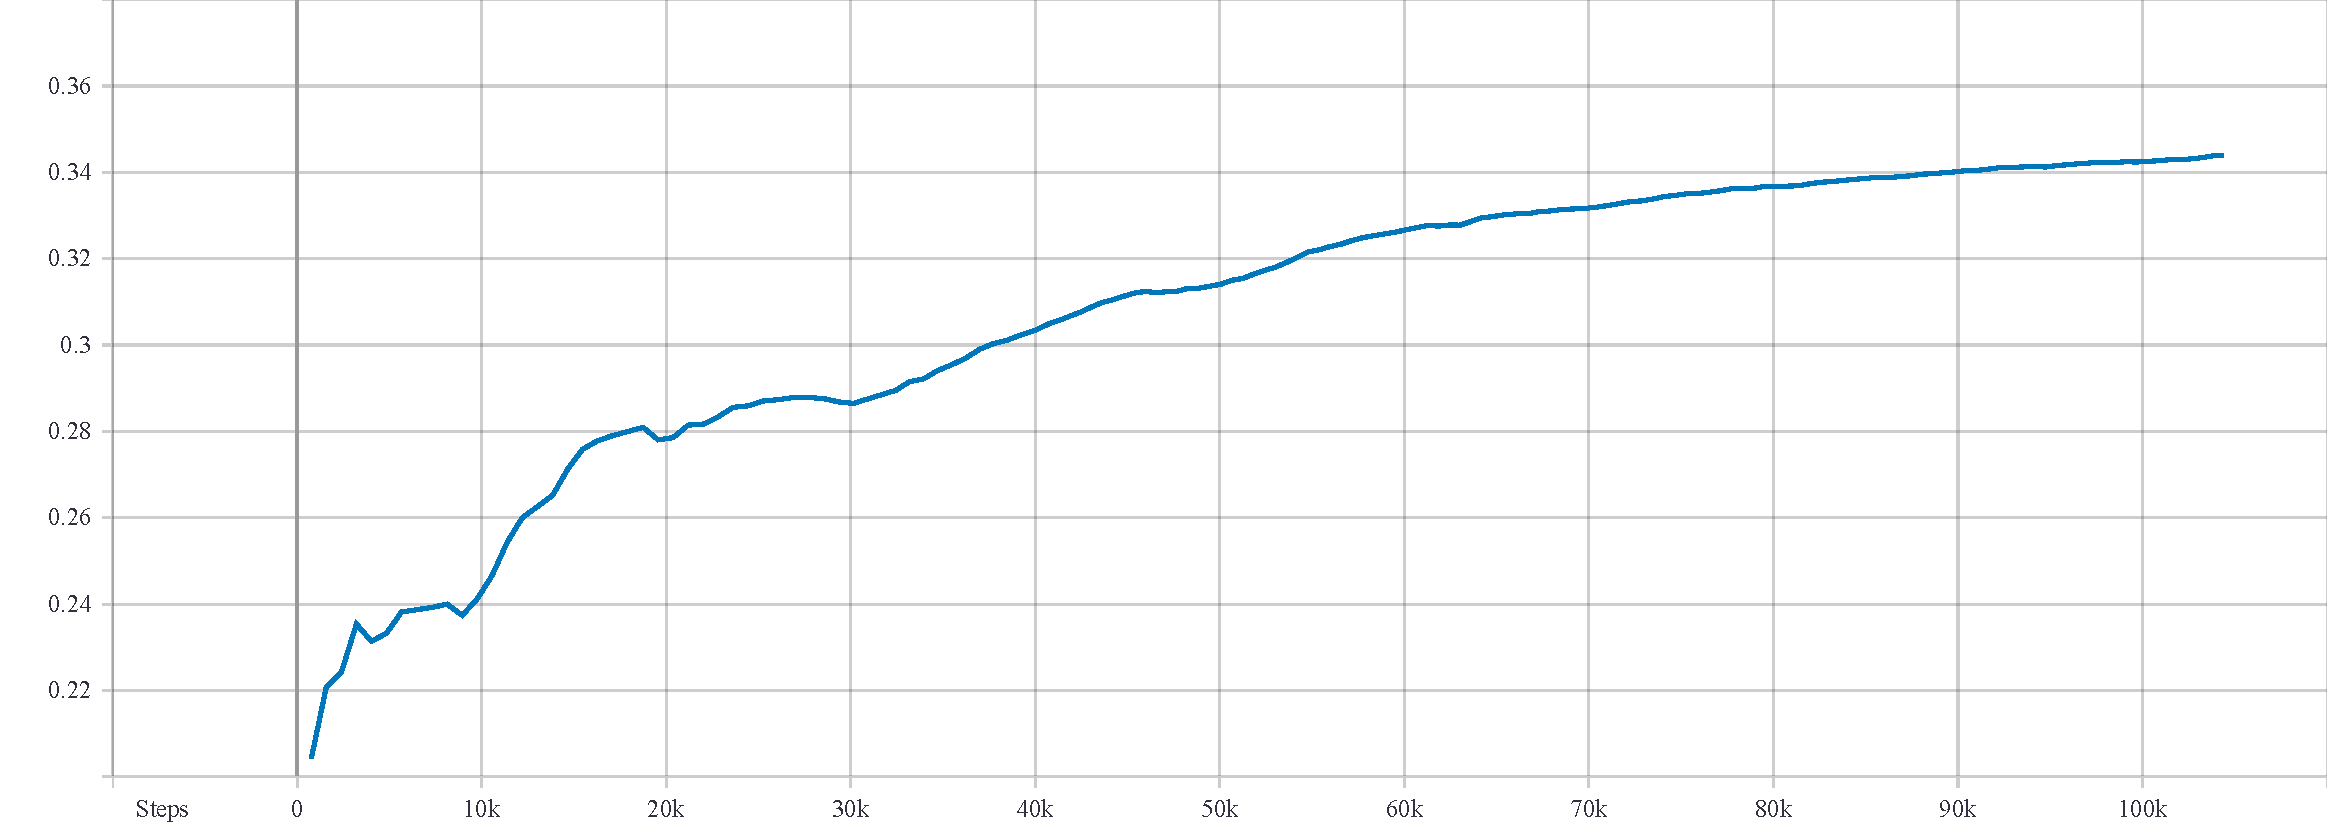
\includegraphics[width=\textwidth]{mAP-75-IoU}
                \caption{Changes of Precision at Different Training Steps for 75\% IoU}
                \label{fig:precision_iou75}
            \end{figure}
            
            \begin{figure}
                \centering
                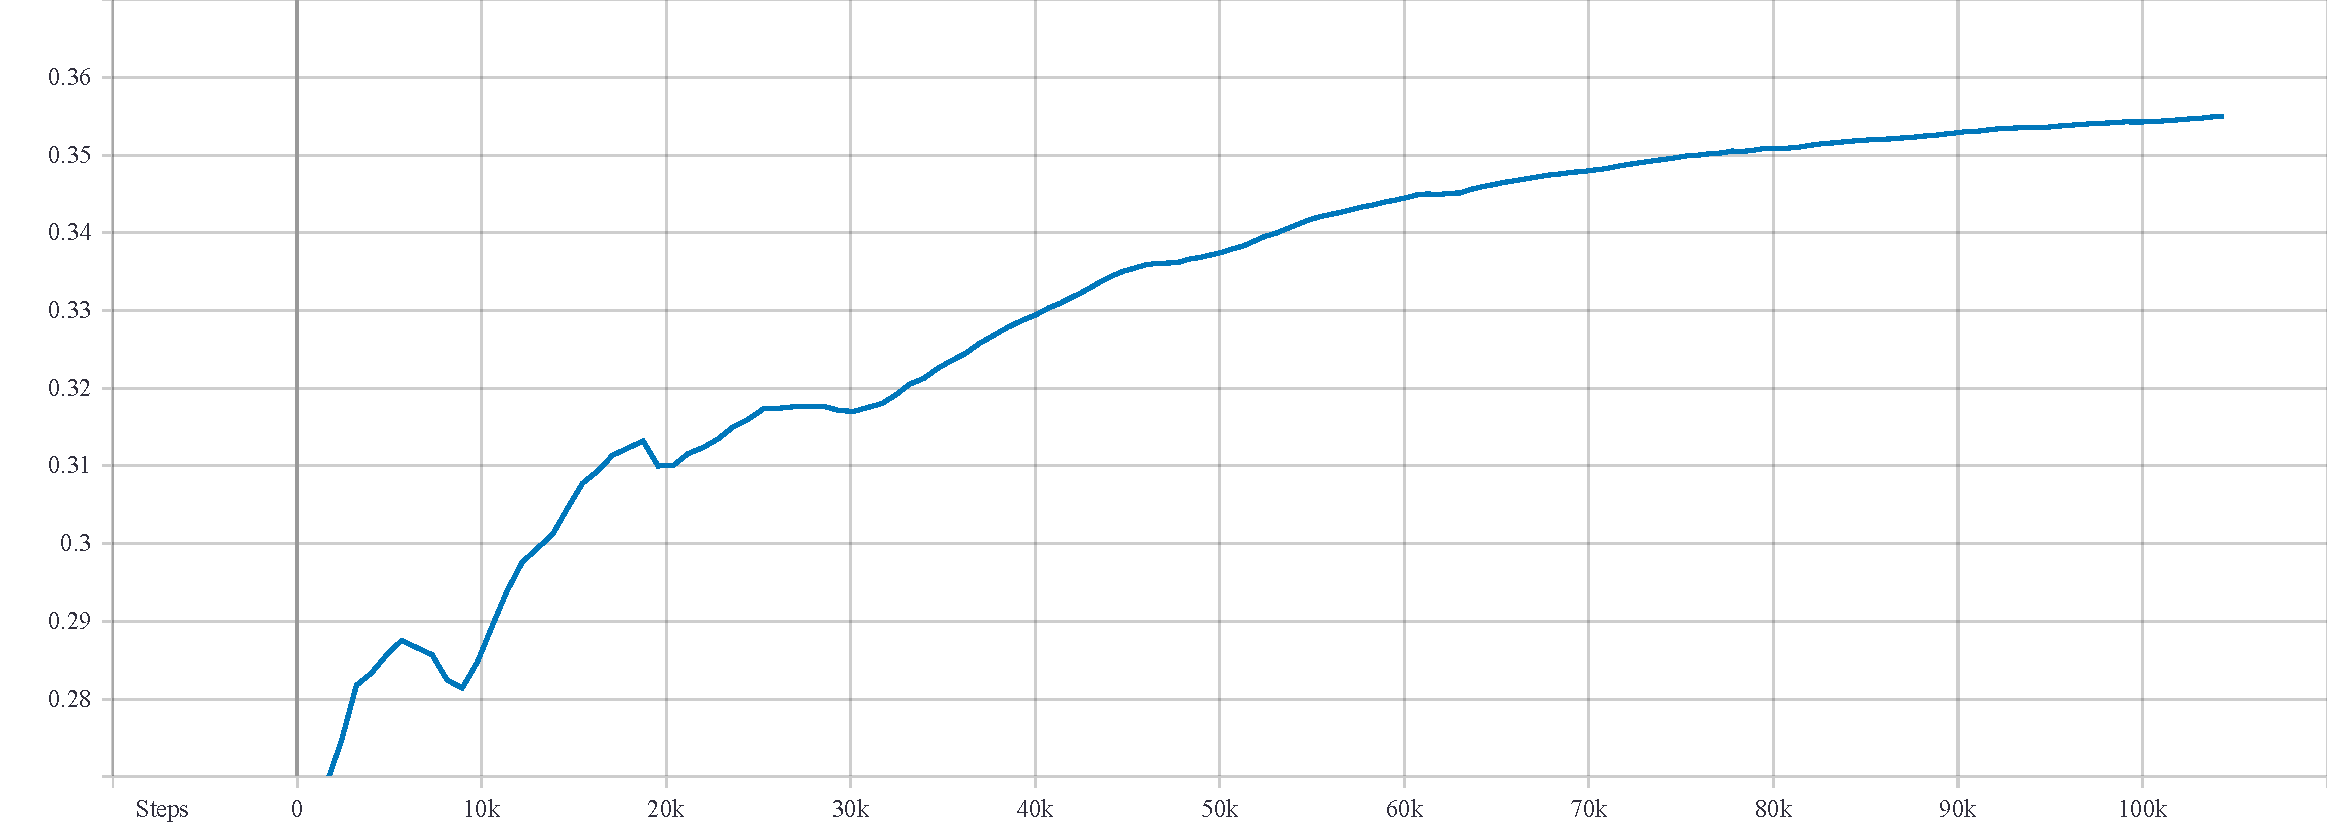
\includegraphics[width=\textwidth]{mAP}
                \caption{Training Steps vs Precision for 50\%:5\%:95\% IoU}
                \label{fig:precision_ioucoco}
            \end{figure}
            
            \begin{figure}
                \centering
                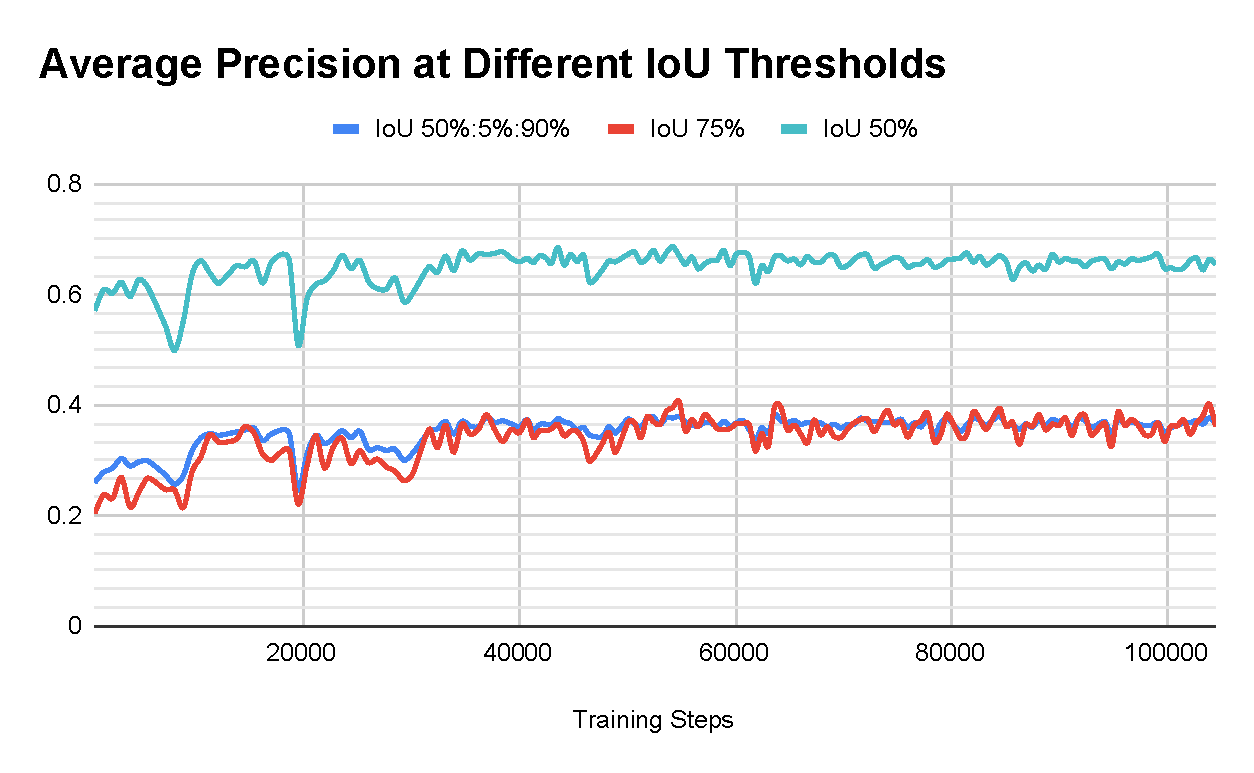
\includegraphics[width=\textwidth]{Average-Precision-at-Different-IoU-Thresholds}
                \caption{Changes of Precision for Different IoU (Compared)}
                \label{fig:precision_iou}
            \end{figure}
            
            \begin{table}
                \centering
                \begin{tabular}{|c||c|} \hline 
                     IoU Threshold  &  Precision on Validation Data \\\hline\hline
                     50\%  &  0.65 \\\hline
                     75\%  &  0.36 \\\hline
                     50\%:5\%:90\%  &  0.37 \\\hline
                \end{tabular}
                \caption{Precision at Different IoU Thresholds}
                \label{tab:precision_iou}
            \end{table}
            
        \clearpage
        \subsection{Average Precision for Different Pothole-Sizes}
            Here, we show the model's performance taking the Average Precision considering different occupying area-sizes of potholes in the validation images.
            % These values are shown in Table \ref{tab:precision_sizes}. The full history of changes at different training steps are shown in Figure \ref{fig:precision_sizes}.
            
            \begin{figure}[h]
                \centering
                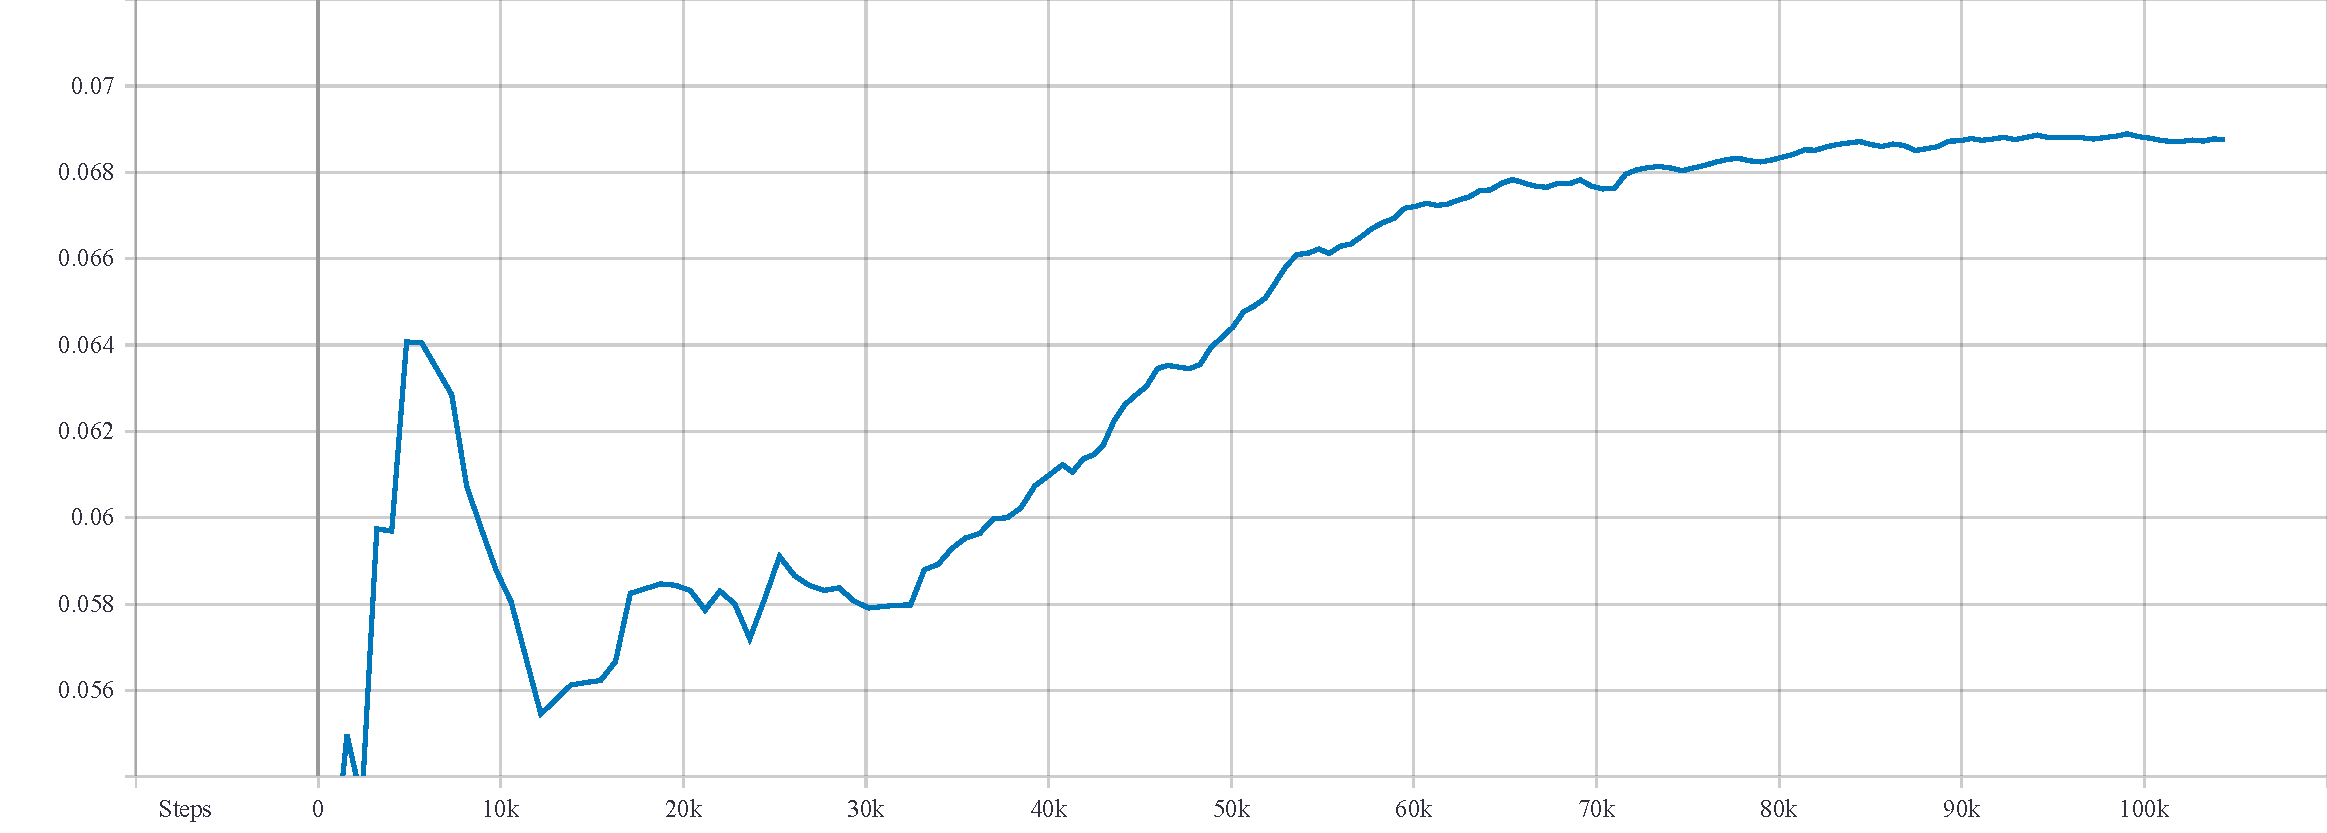
\includegraphics[width=\textwidth]{mAP-small}
                \caption{Changes of Precision-Values for Small Potholes}
                \label{fig:precision_sizes_small}
            \end{figure}
            
            \begin{figure}[h]
                \centering
                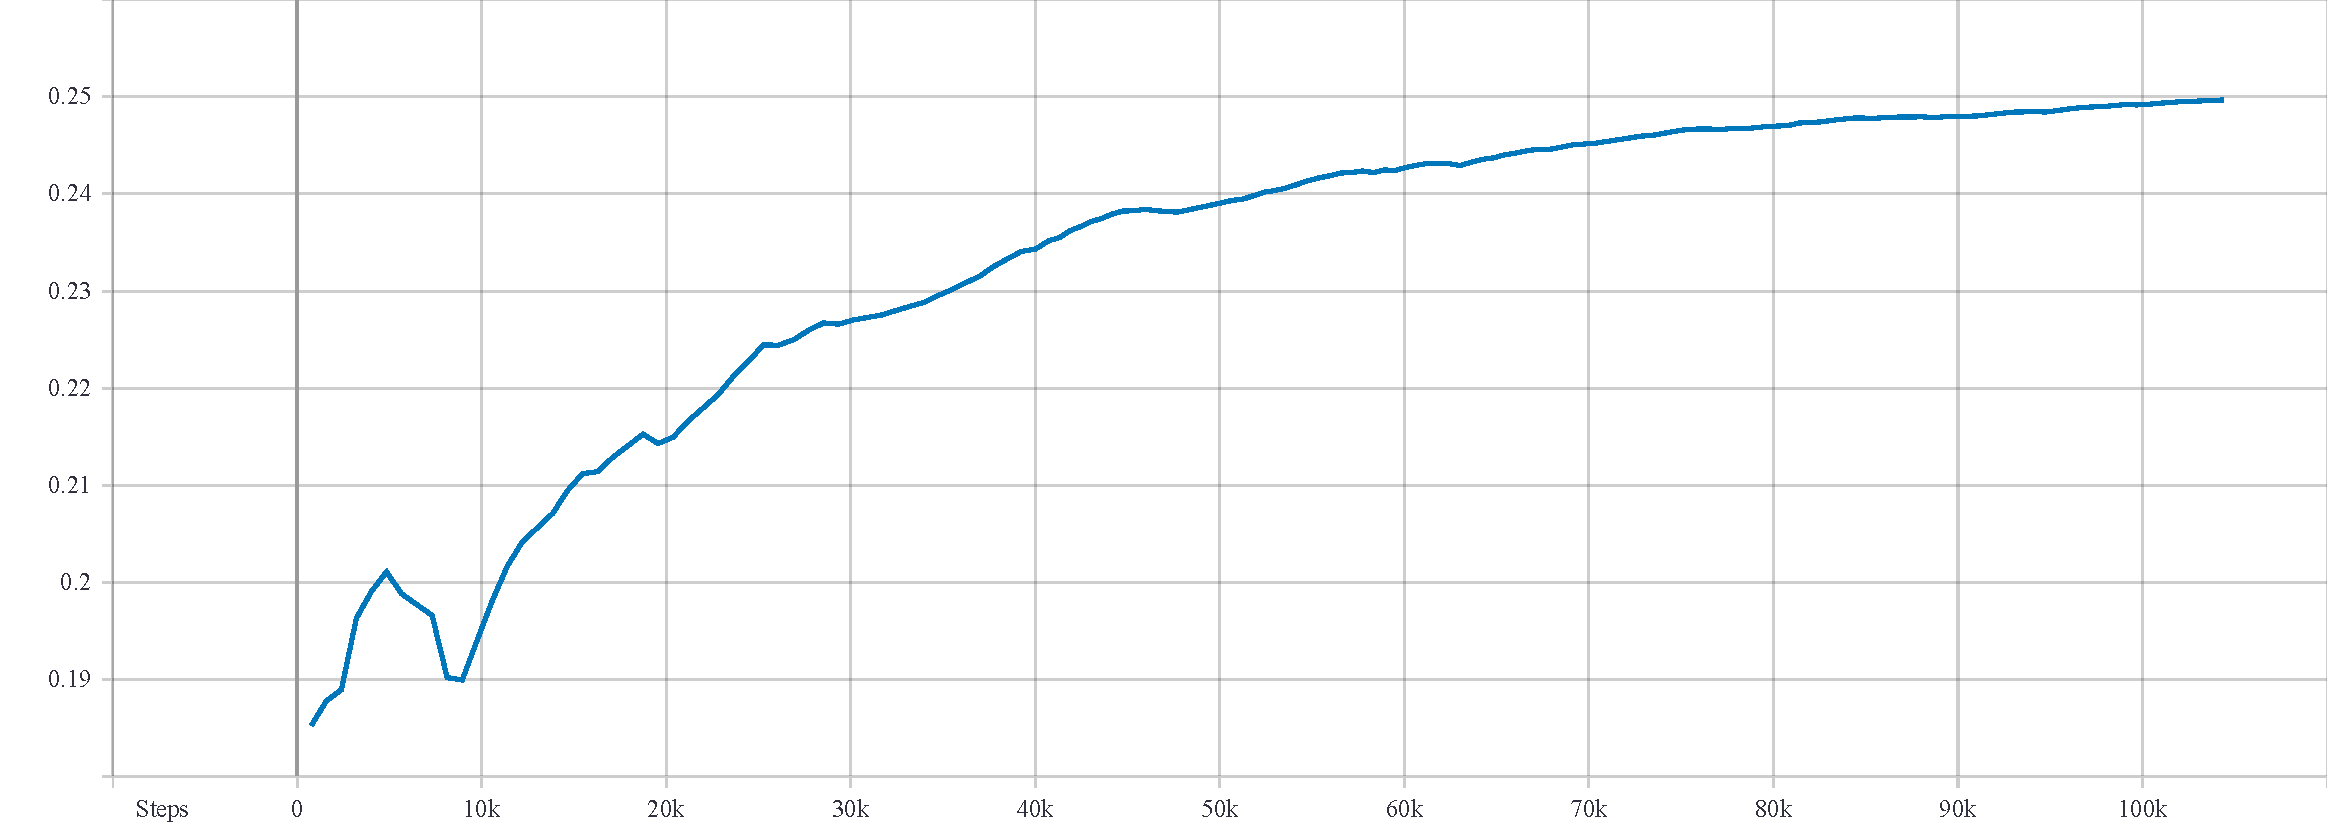
\includegraphics[width=\textwidth]{mAP-medium}
                \caption{Changes of Precision-Values for Medium Potholes}
                \label{fig:precision_sizes_medium}
            \end{figure}
            
            \begin{figure}
                \centering
                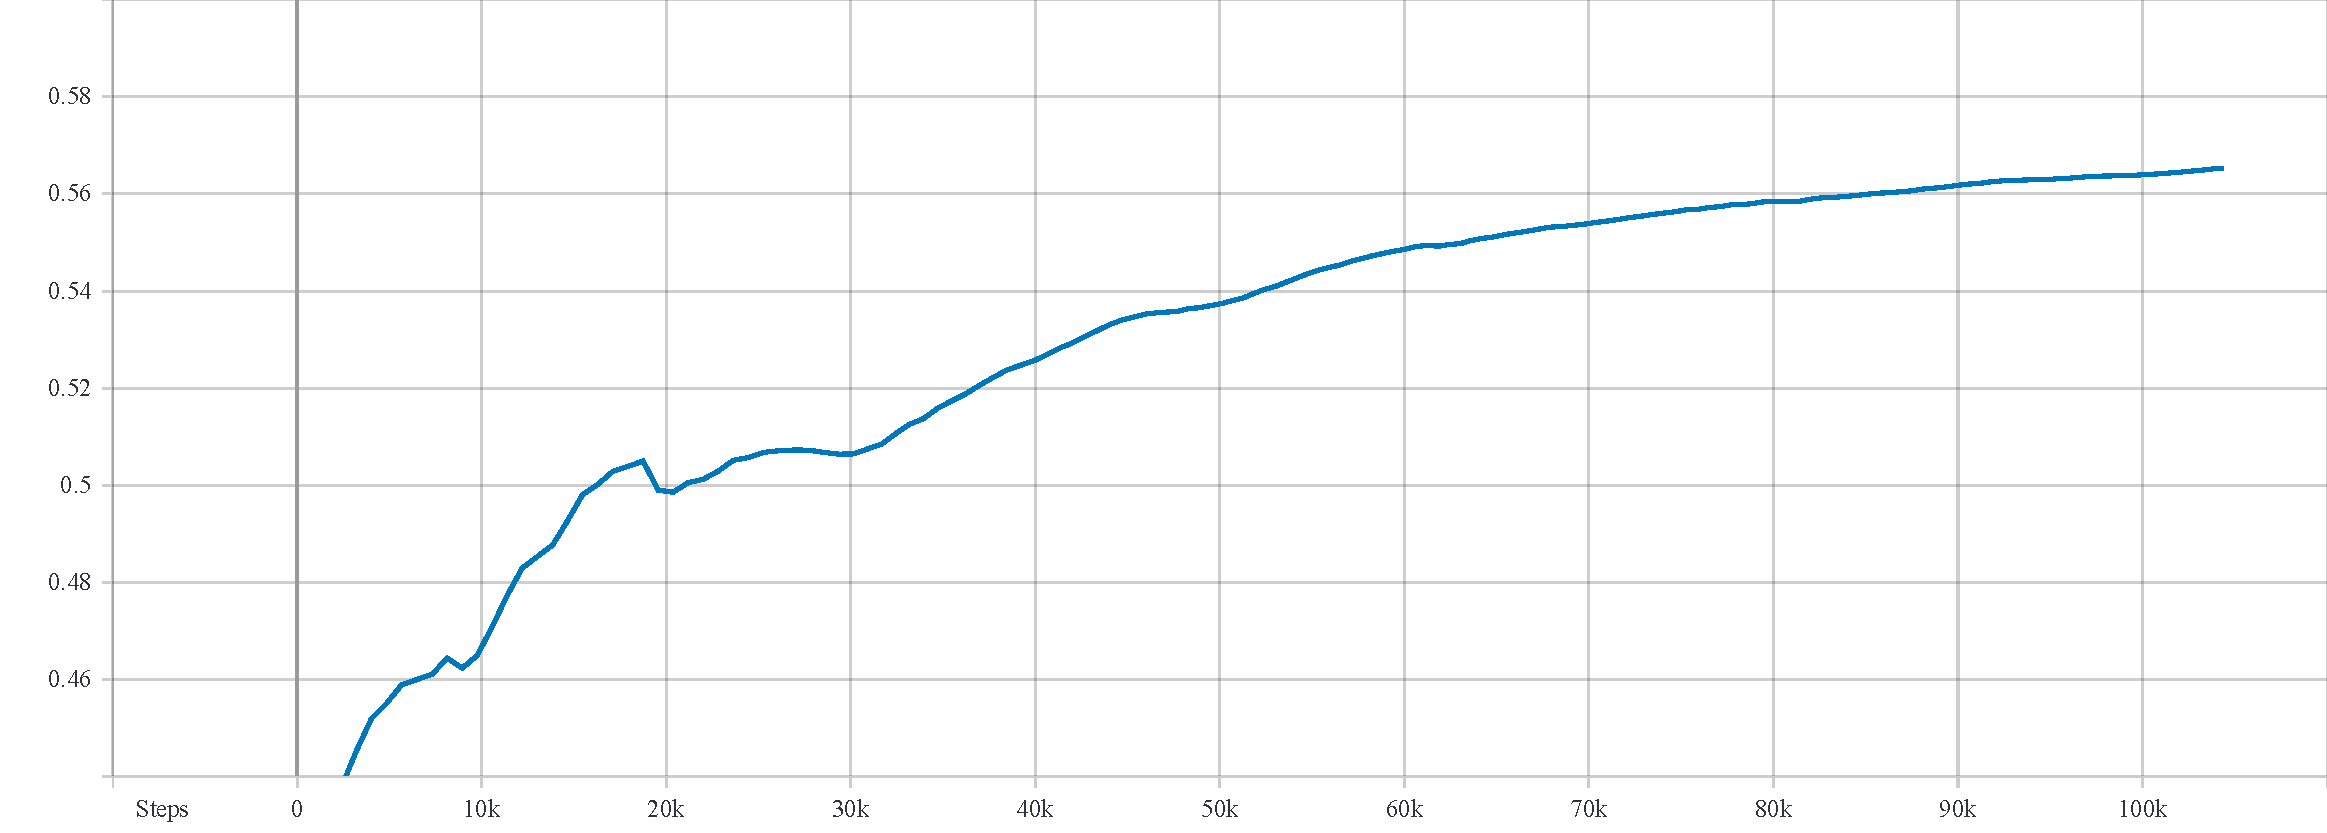
\includegraphics[width=\textwidth]{mAP-large}
                \caption{Changes of Precision-Values for Large Potholes}
                \label{fig:precision_sizes_large}
            \end{figure}
            
            \begin{table}
                \centering
                \begin{tabular}{|c||c|} \hline 
                     Area Sizes  &  Precision on Validation Data \\\hline\hline
                     Small  &  0.07 \\\hline
                     Medium  &  0.26 \\\hline
                     Large  &  0.58 \\\hline
                \end{tabular}
                \caption{Precision for Different Pothole-Sizes}
                \label{tab:precision_sizes}
            \end{table}
            
            \clearpage
            \begin{figure}
                \centering
                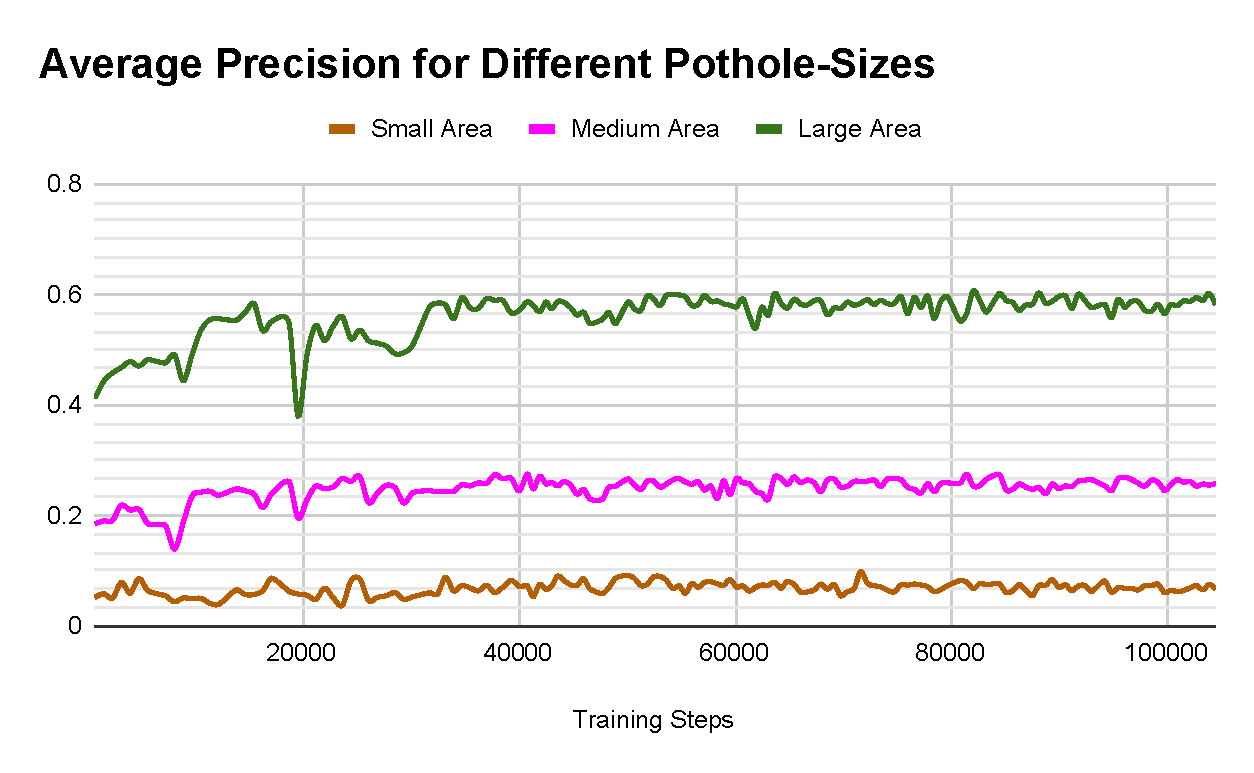
\includegraphics[width=\textwidth]{Average-Precision-for-Different-Pothole-Sizes}
                \caption{Training-Steps vs Precision for Different Pothole-Sizes (Compared)}
                \label{fig:precision_sizes}
            \end{figure}
            
            \begin{figure}
                \centering
                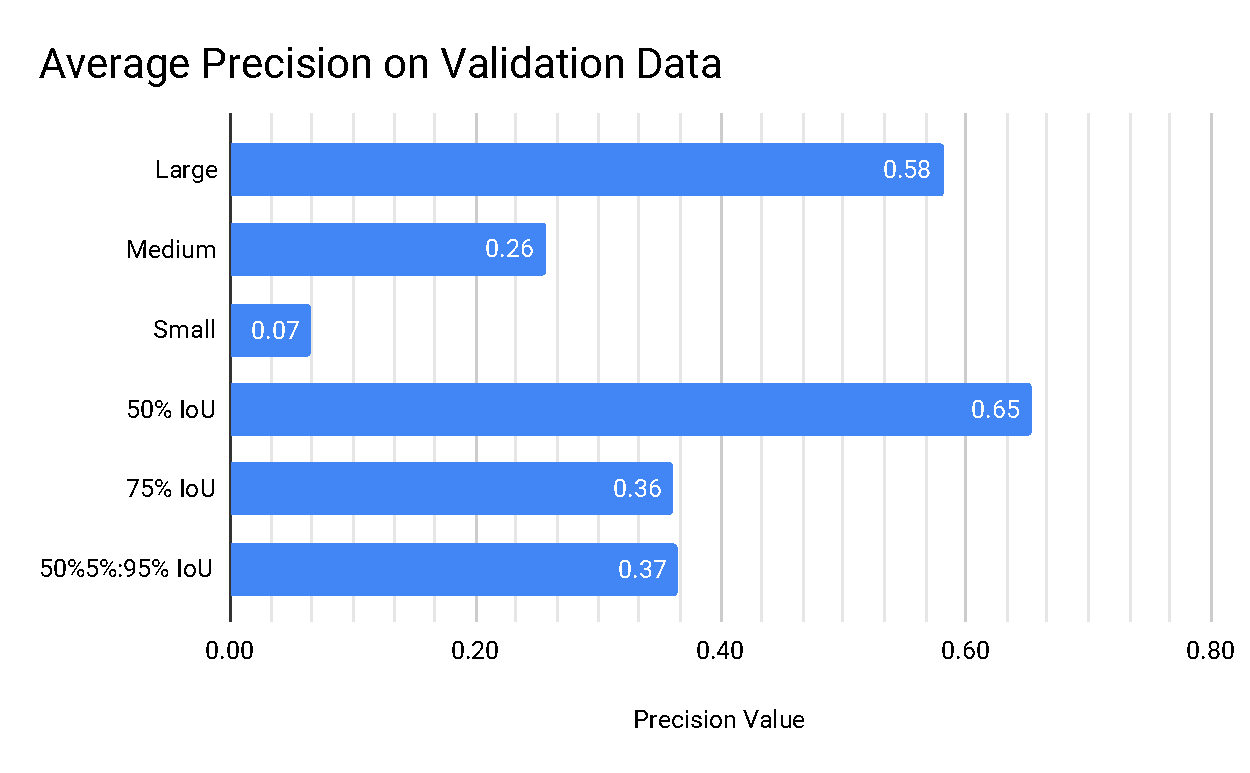
\includegraphics[width=\textwidth]{Average-Precision-on-Validation-Data}
                \caption{Validation Average-Precision (All Compared)}
                \label{fig:precisions}
            \end{figure}
            
    \clearpage
    \section{Recall at Different Training Steps}
        Recall is a good parameter for the evaluation of the performance of a model. While the training process was running for our model, we have triggered the evaluation function at different checkpoints. We have found a history of how the recall values changed according to the training steps. Finally, we calculated the overall and final recall values for different thresholds. We took different detection limits and different area-sizes of potholes in validation images.
        
        \subsection{Average Recall at Different Detection Limits}
            Recall is actually valid when the limit is defined. That is, upto how many detections it is being calculated should be explicitly stated.
            
            \vspace{1cm}
            We have taken the recall values at different limits of maximum detections. More specifically, we have taken the following limits for the calculation of recall values---
            \begin{enumerate}
                \item {Average Recall at maximum of 1 detection (AR@1)}
                \item {Average Recall at maximum of 10 detections (AR@10)}
                \item {Average Recall at maximum of 100 detection (AR@100)}
            \end{enumerate}
            
            \vspace{1cm}
            To visualize the history of how the recall values changed throughout the whole training process the Figure \ref{fig:recall_limits} can be referred to. This figure generated from running inference on the validation images at different training stages.
            
            \vspace{1cm}
            From table \ref{tab:recall_limits}, it can bee seen that the overall and final values the model yielded after the training process has exceeded 100,000 steps. This large number of steps for training can be considered to take the recall values at a high level of acceptance.
            
            \clearpage
            \begin{figure}
                \centering
                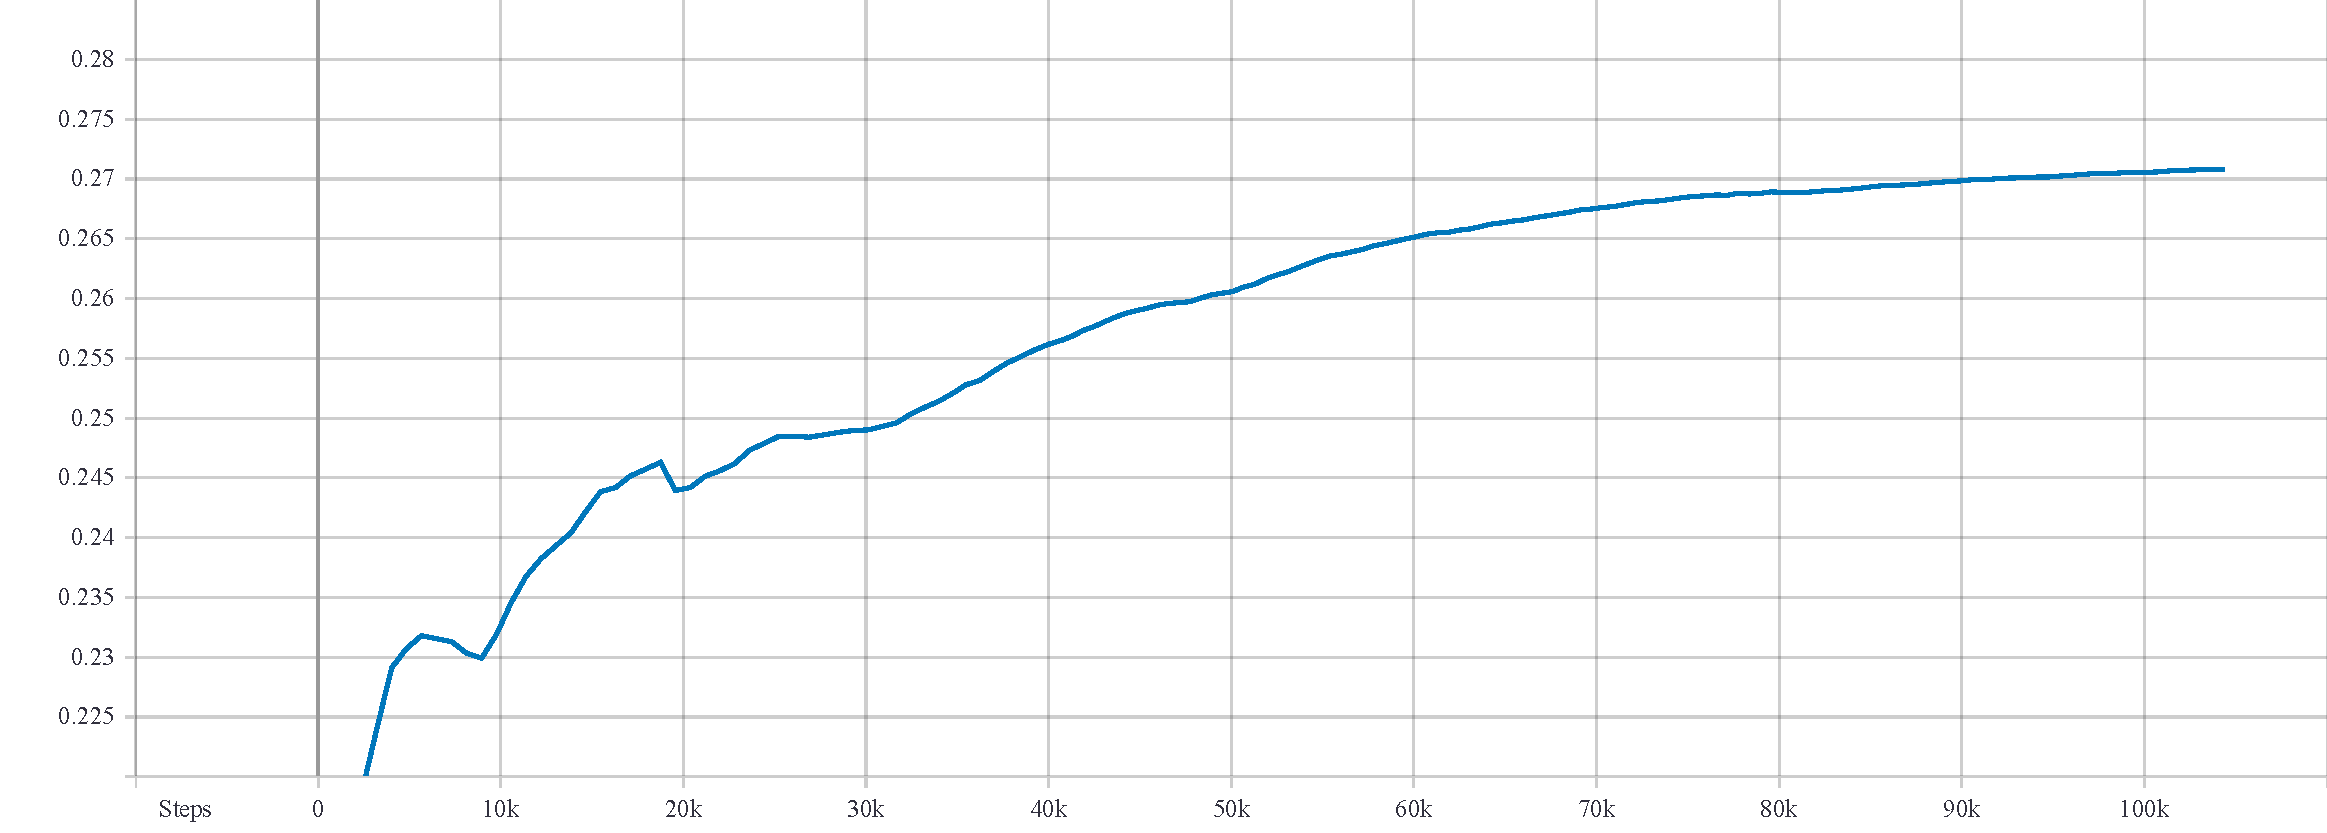
\includegraphics[width=\textwidth]{AR-1}
                \caption{Changes of Recall-Values for Max 1 Detection}
                \label{fig:recall_limits_1}
            \end{figure}
            \begin{figure}
                \centering
                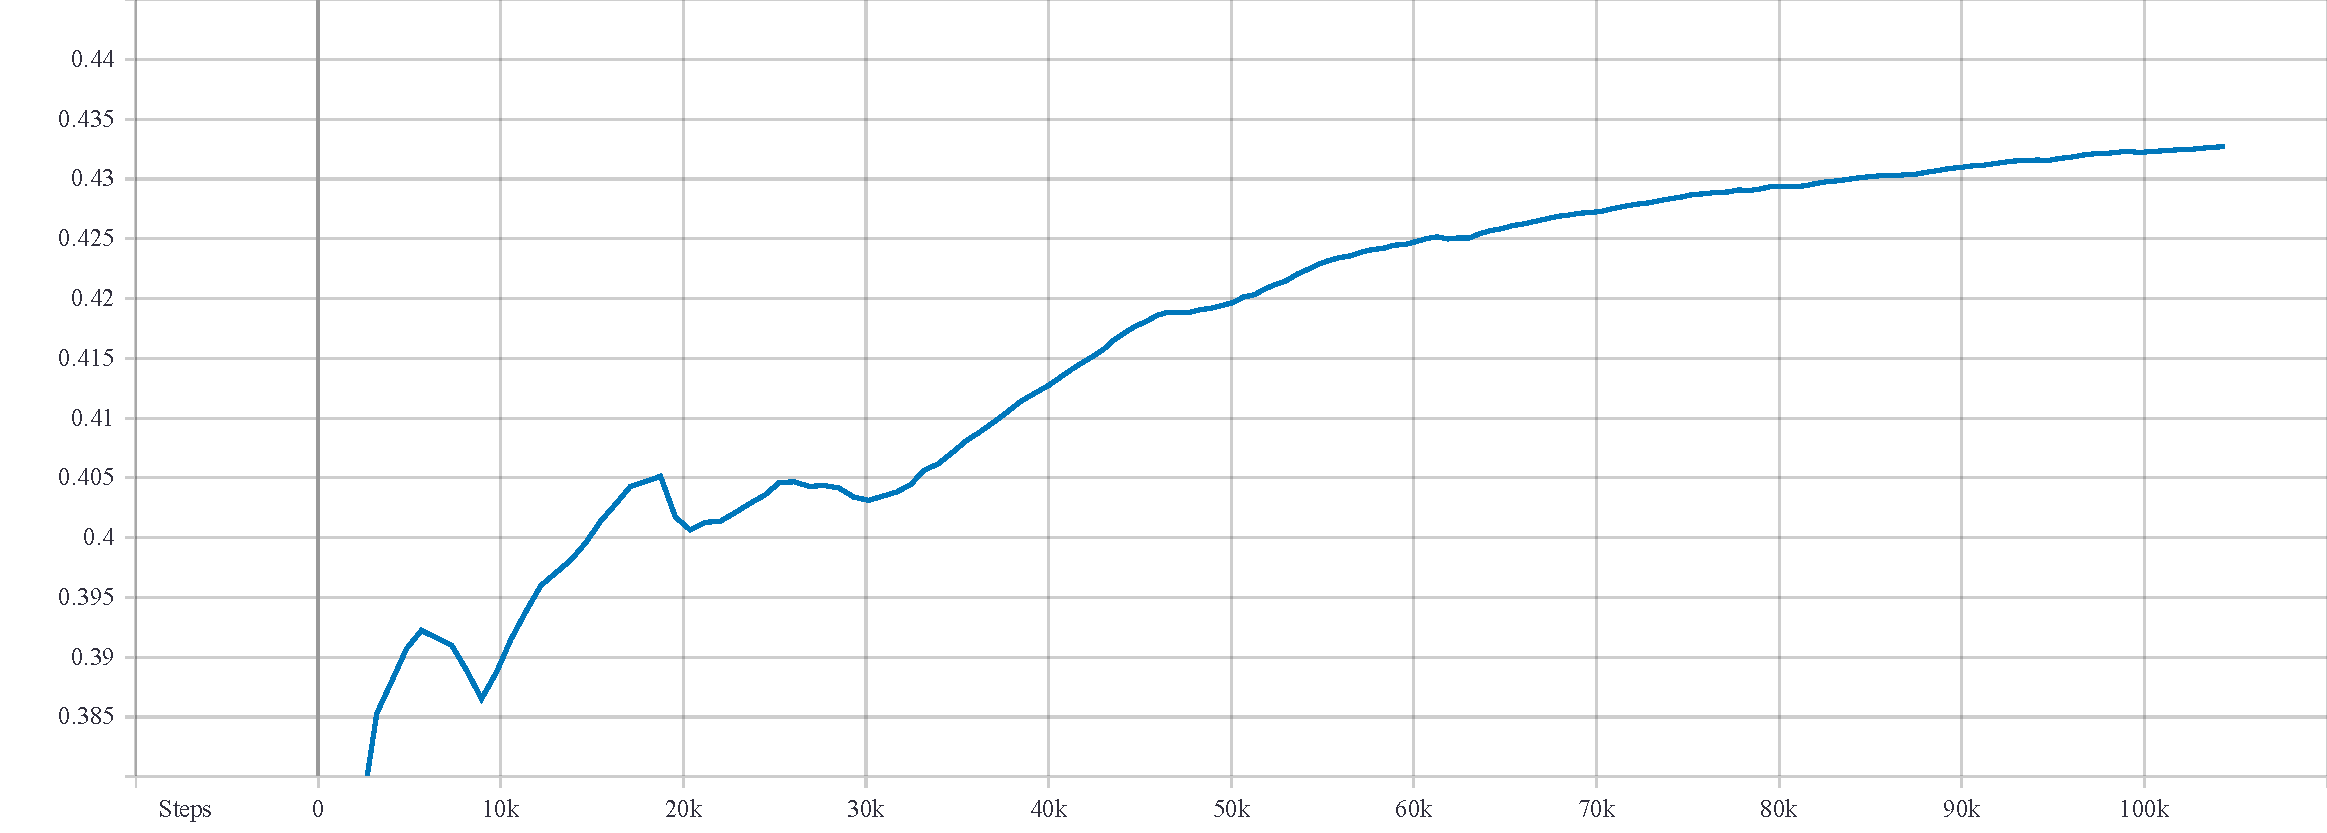
\includegraphics[width=\textwidth]{AR-10}
                \caption{Changes of Recall-Values for Max 10 Detections}
                \label{fig:recall_limits_10}
            \end{figure}
            \begin{figure}
                \centering
                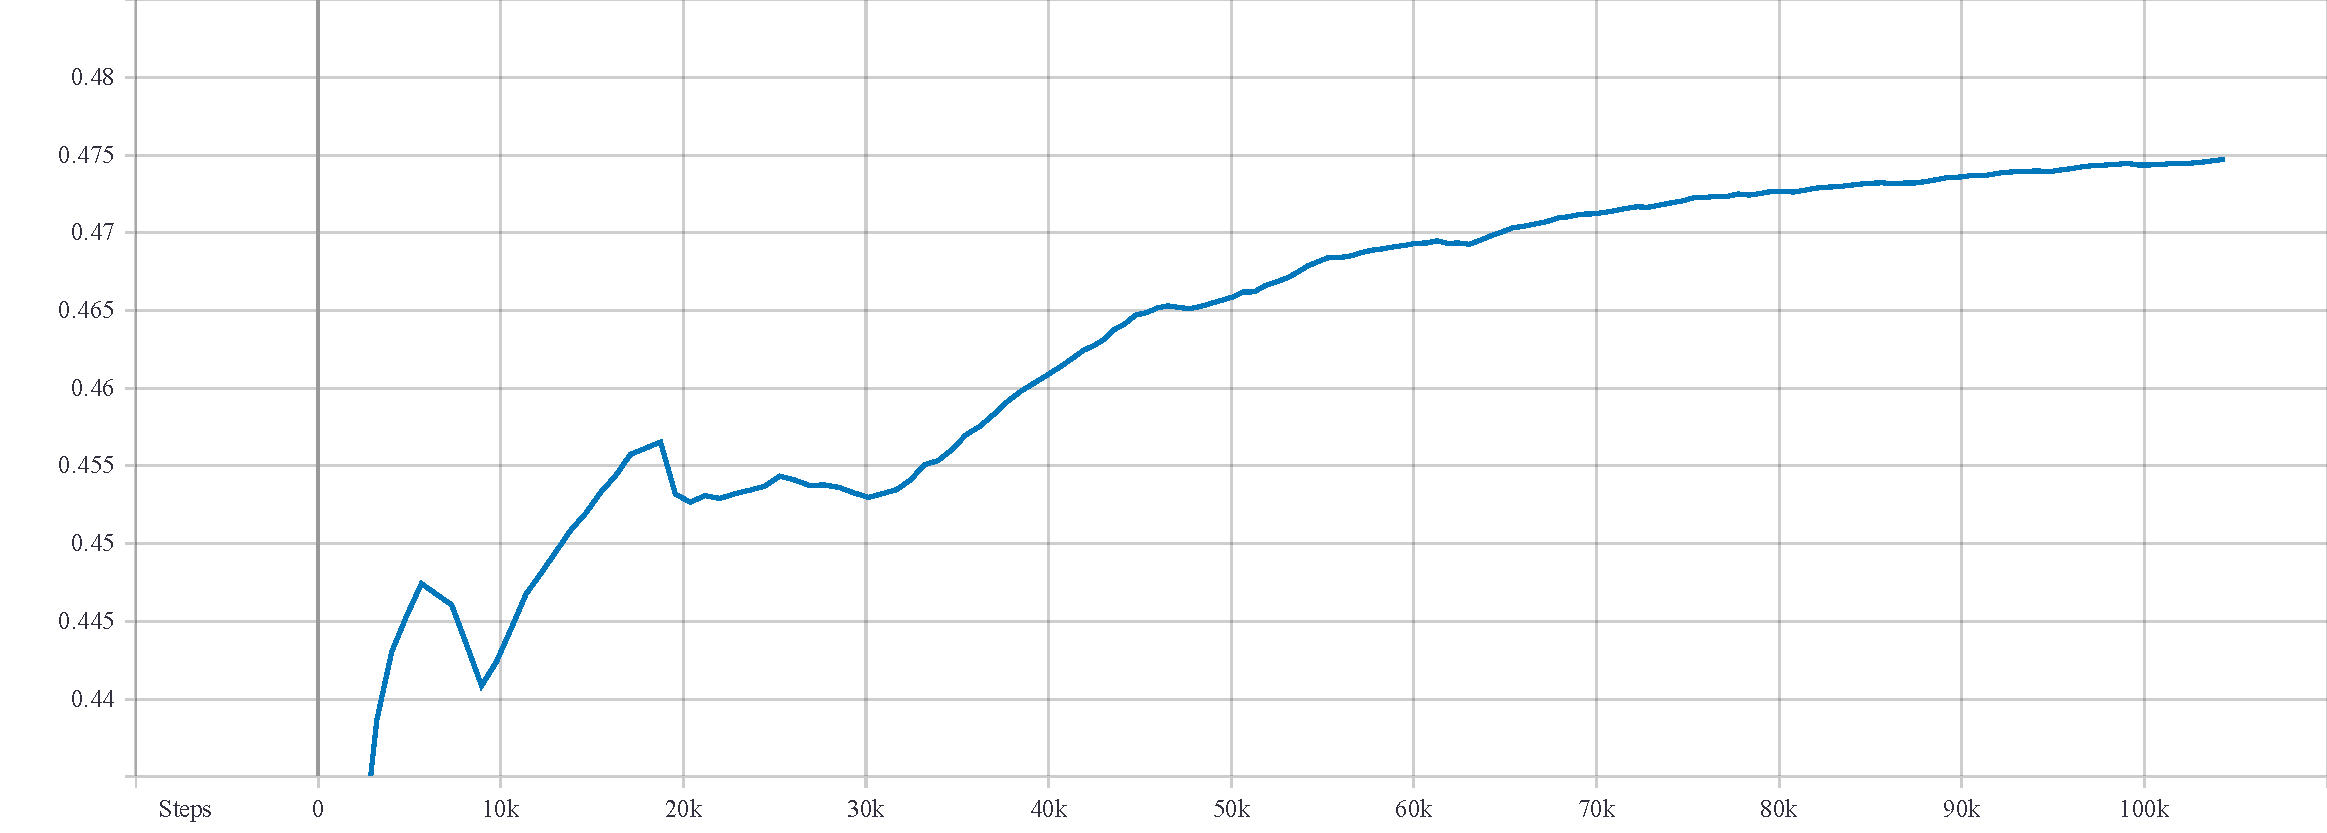
\includegraphics[width=\textwidth]{AR-100}
                \caption{Changes of Recall-Values for Max 100 Detections}
                \label{fig:recall_limits_100}
            \end{figure}
            
            \begin{figure}
                \centering
                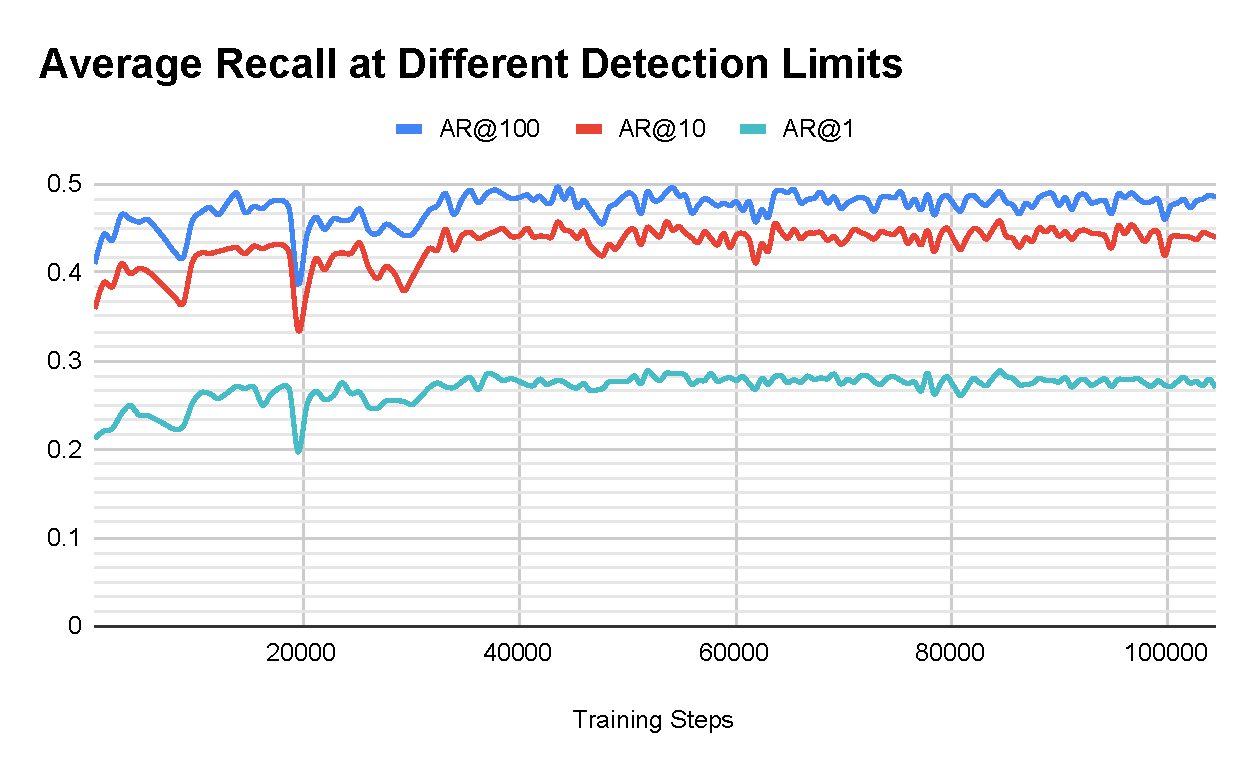
\includegraphics[width=\textwidth]{Average-Recall-at-Different-Detection-Limits}
                \caption{Changes of Recall-Values for Different Detection-Limits}
                \label{fig:recall_limits}
            \end{figure}
            
            \begin{table}
                \centering
                \begin{tabular}{|c||c|} \hline 
                     Maximum Detections  &  Recall on Validation Data \\\hline\hline
                     1  &  0.27 \\\hline
                     10  &  0.44 \\\hline
                     100  &  0.49 \\\hline
                \end{tabular}
                \caption{Recall for Different Detection-Limits}
                \label{tab:recall_limits}
            \end{table}
            
        \clearpage
        \subsection{Average Recall for Different Pothole-Sizes}
            Our model was evaluated against recall values taken for different sizes of potholes---
            \begin{enumerate}
                \item {Small: $Image\-Area < 32^2 px$}
                \item {Medium: $32^2 px \leq Image\-Area \leq 96^2 px$}
                \item {Large: $Image\-Area > 96^2 px$}
            \end{enumerate}
            
            \begin{figure}[h]
                \centering
                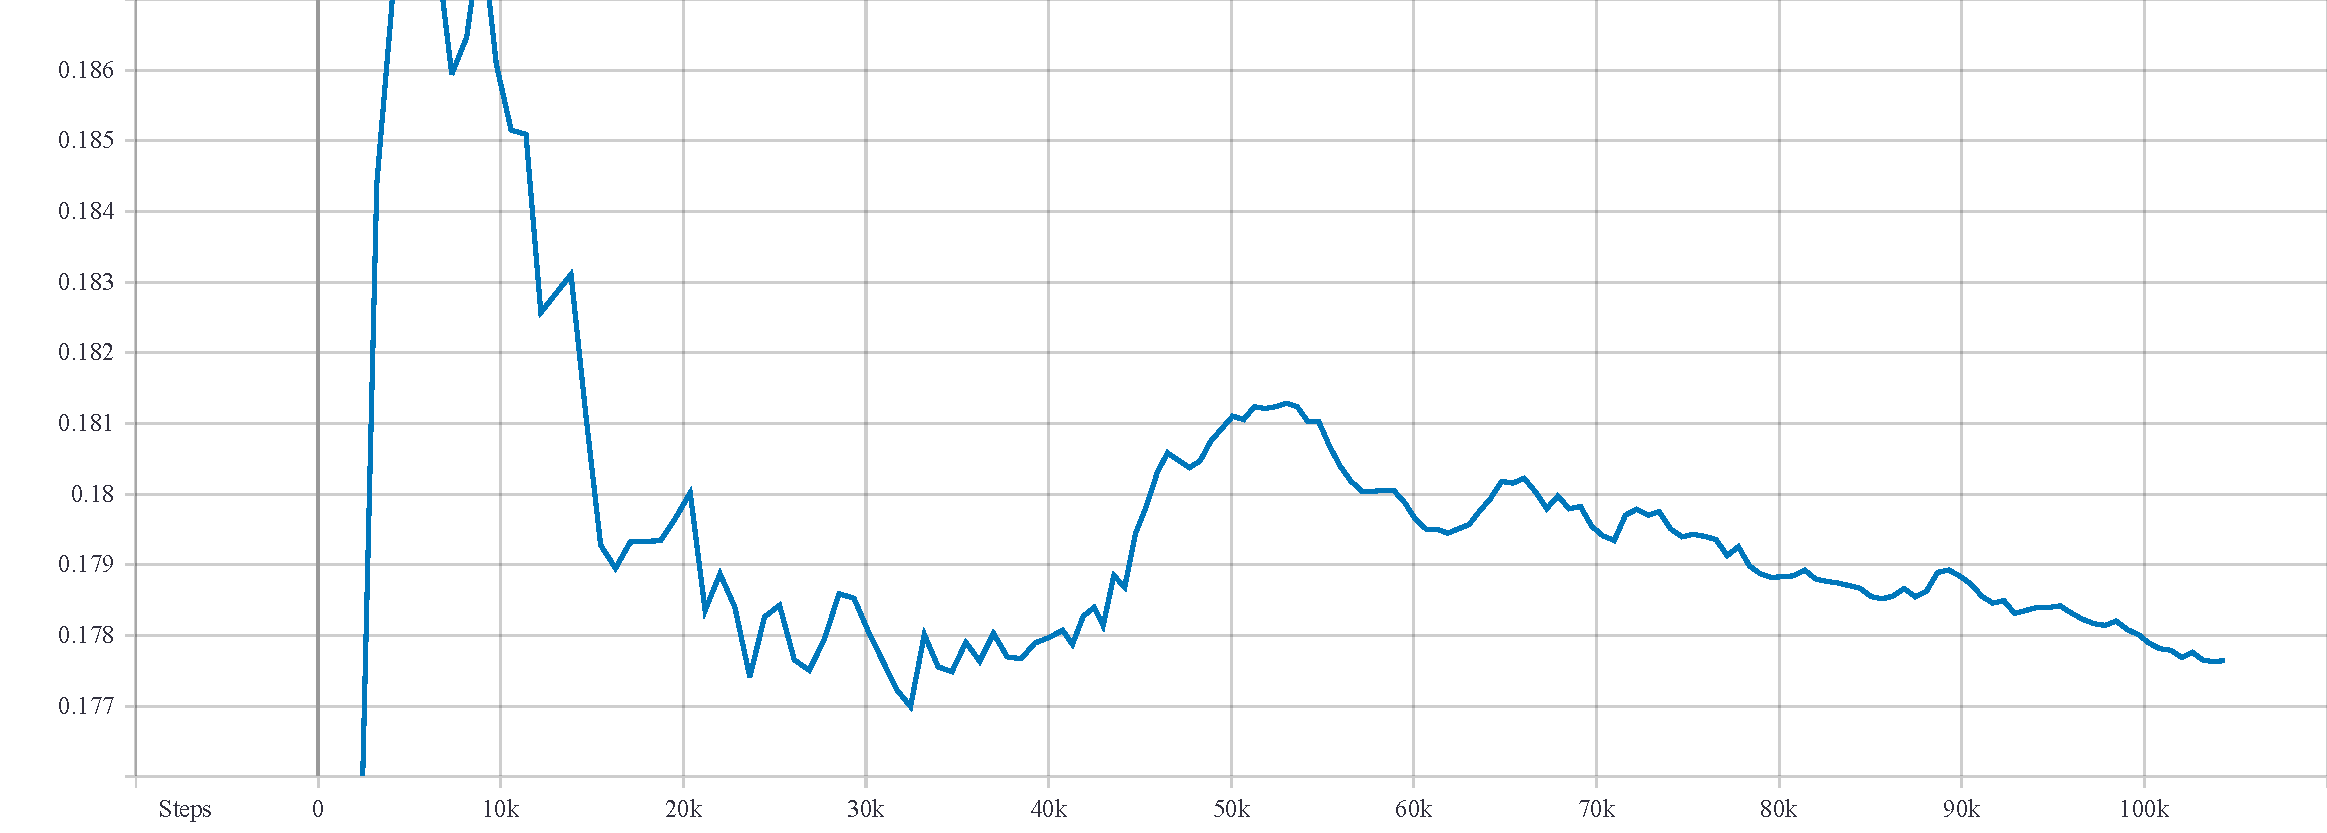
\includegraphics[width=\textwidth]{AR-small}
                \caption{Changes of Recall-Values for Small Potholes}
                \label{fig:recall_size_small}
            \end{figure}
            \begin{figure}[h]
                \centering
                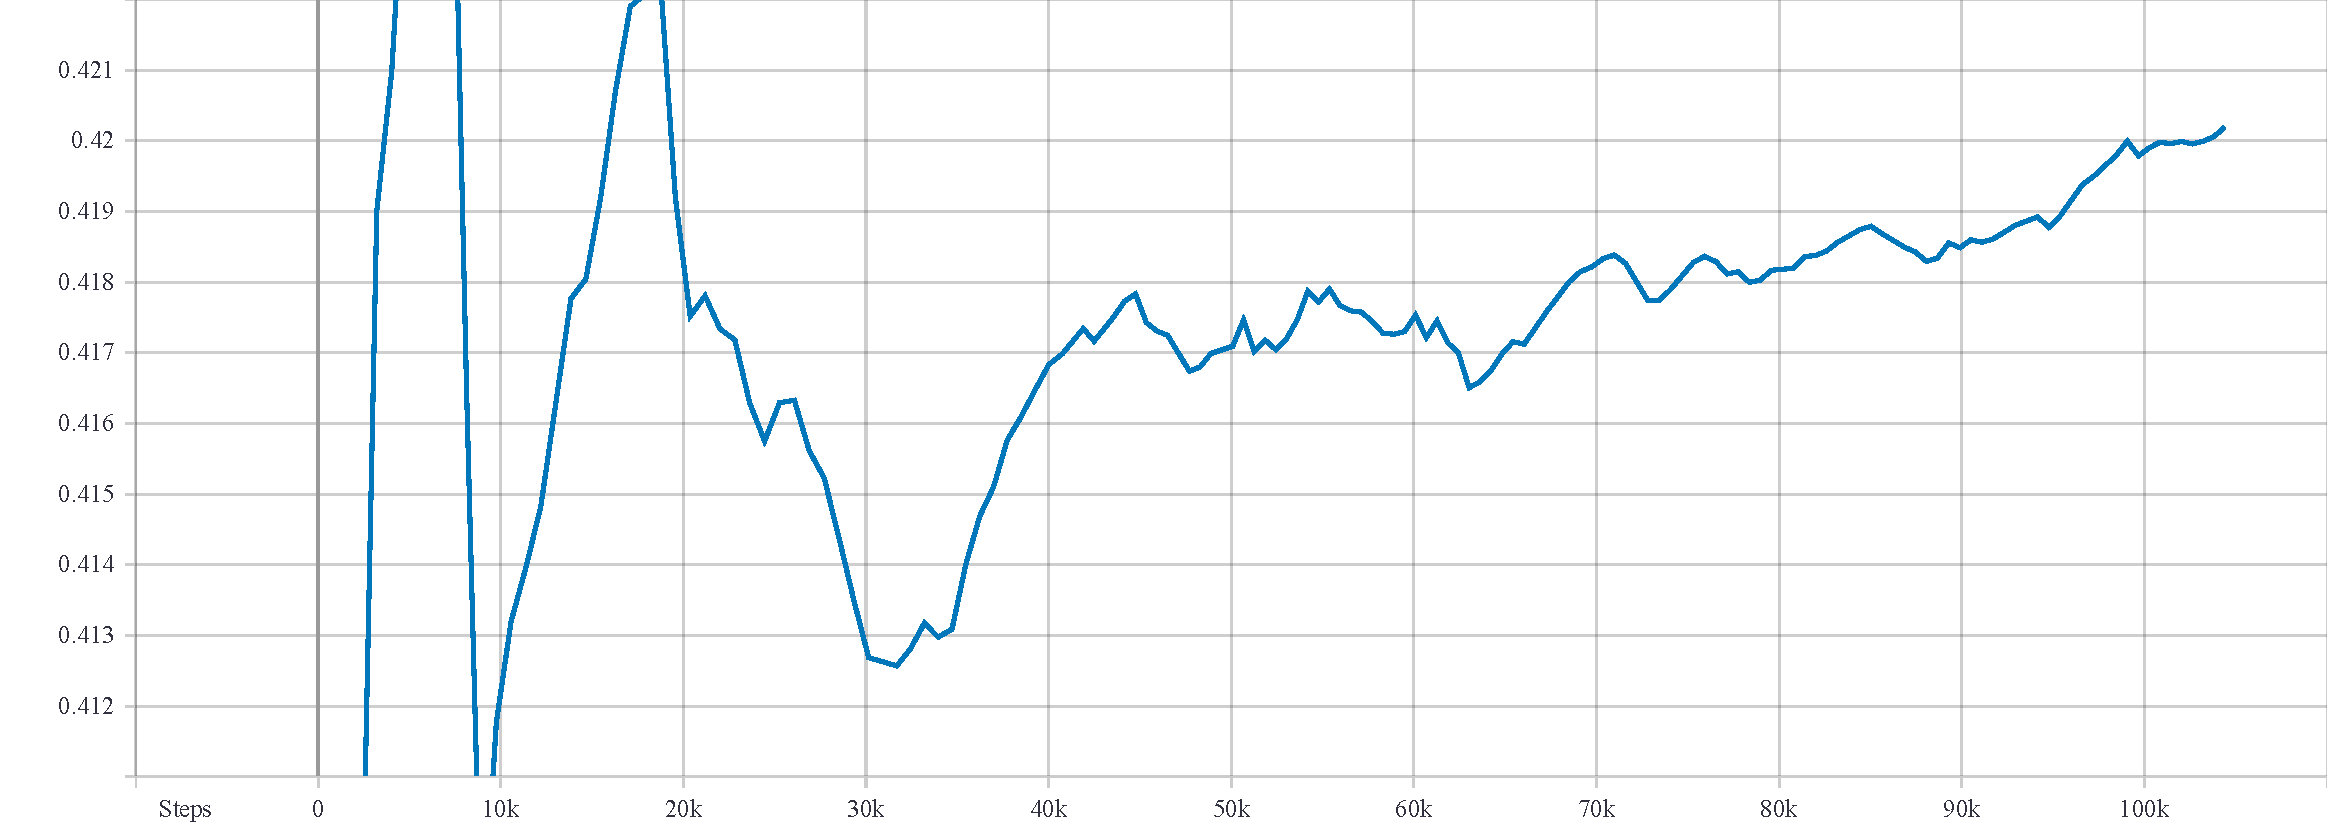
\includegraphics[width=\textwidth]{AR-medium}
                \caption{Changes of Recall-Values for Medium Potholes}
                \label{fig:recall_size_medium}
            \end{figure}
            \begin{figure}
                \centering
                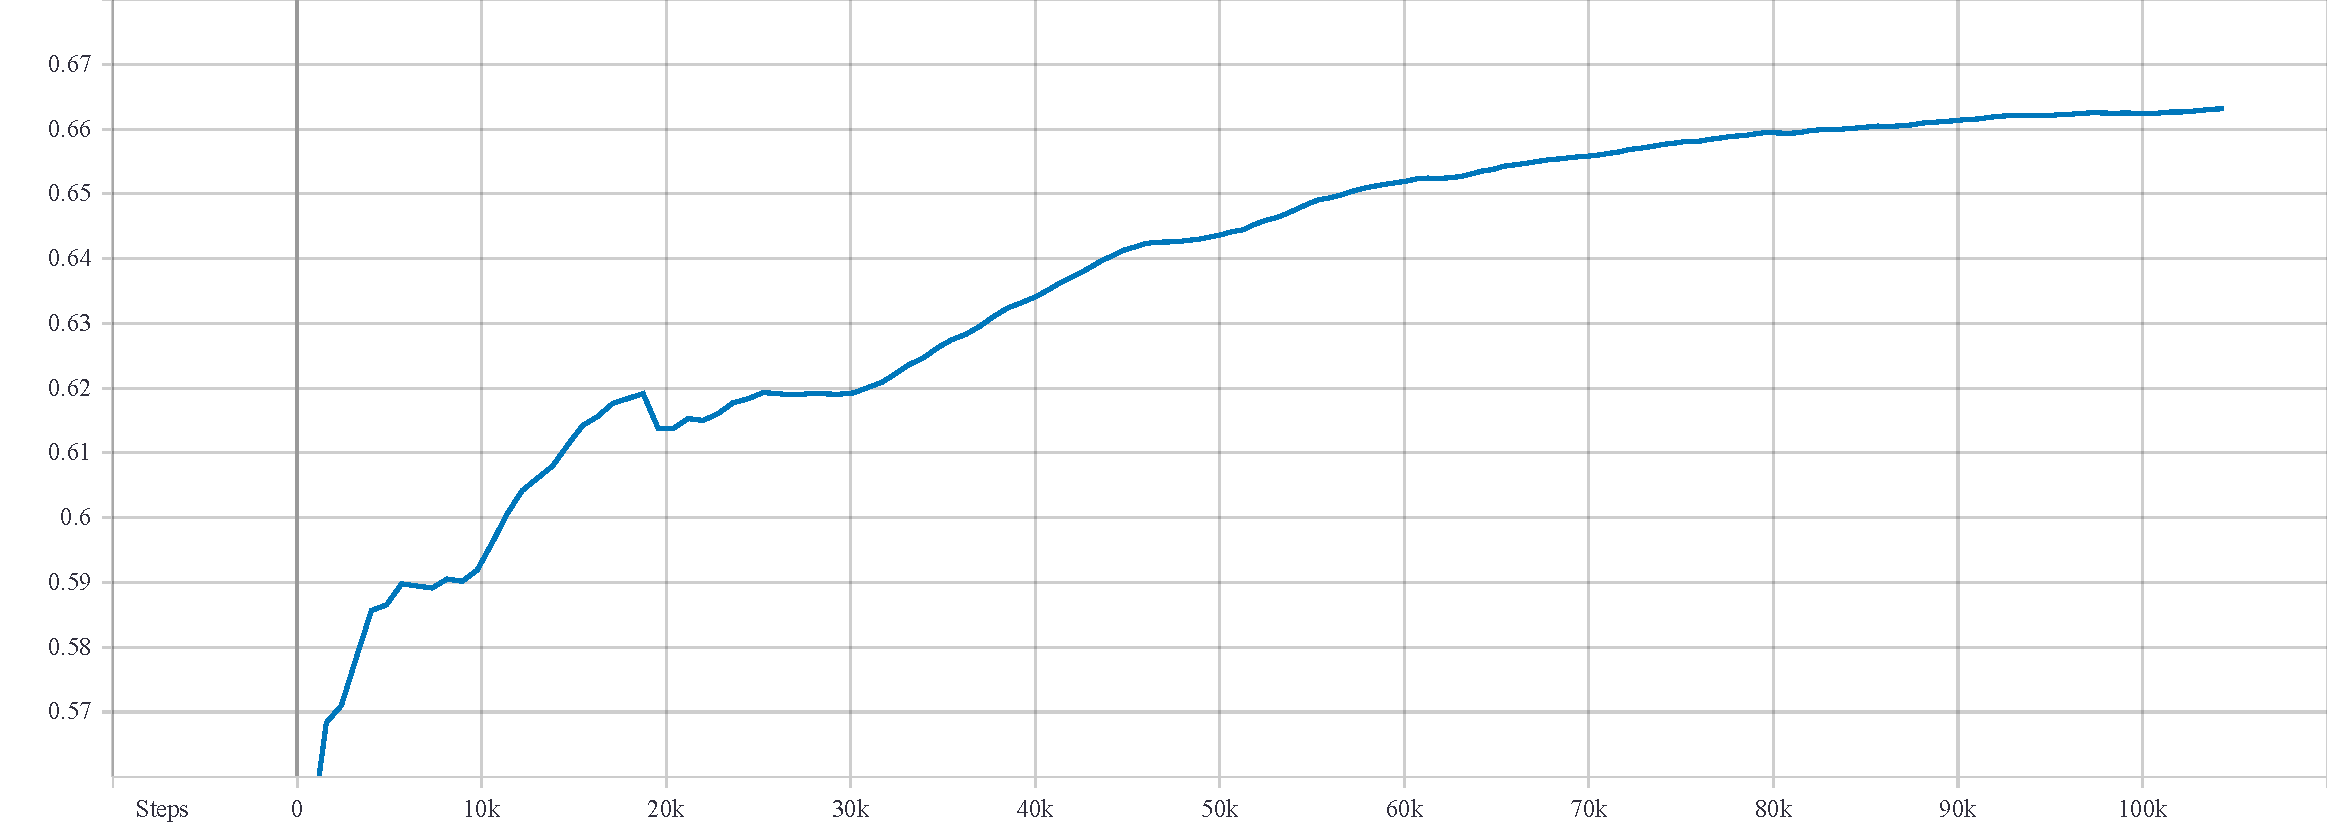
\includegraphics[width=\textwidth]{AR-large}
                \caption{Changes of Recall-Values for Large Potholes}
                \label{fig:recall_size_large}
            \end{figure}
            
            \begin{figure}[ht]
                \centering
                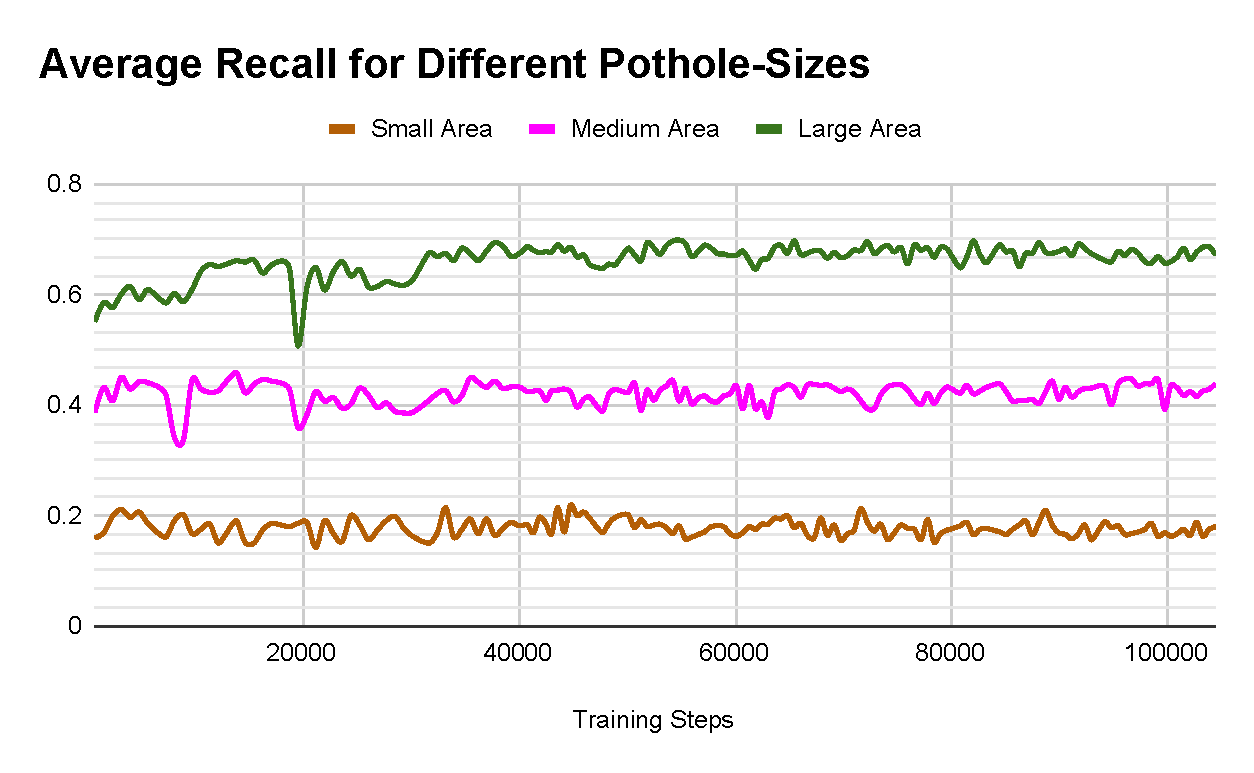
\includegraphics[width=\textwidth]{Average-Recall-for-Different-Pothole-Sizes}
                \caption{Changes of Recall-Values for Different Pothole-Sizes (Compared)}
                \label{fig:recall_sizes}
            \end{figure}
            
            \begin{table}
                \centering
                \begin{tabular}{|c||c|} \hline 
                     Area Sizes  &  Recall on Validation Data \\\hline\hline
                     Small  &  0.18 \\\hline
                     Medium  &  0.44 \\\hline
                     Large  &  0.67 \\\hline
                \end{tabular}
                \caption{Recalls for Different Pothole-Sizes}
                \label{tab:recall_sizes}
            \end{table}
            
            \begin{figure}
                \centering
                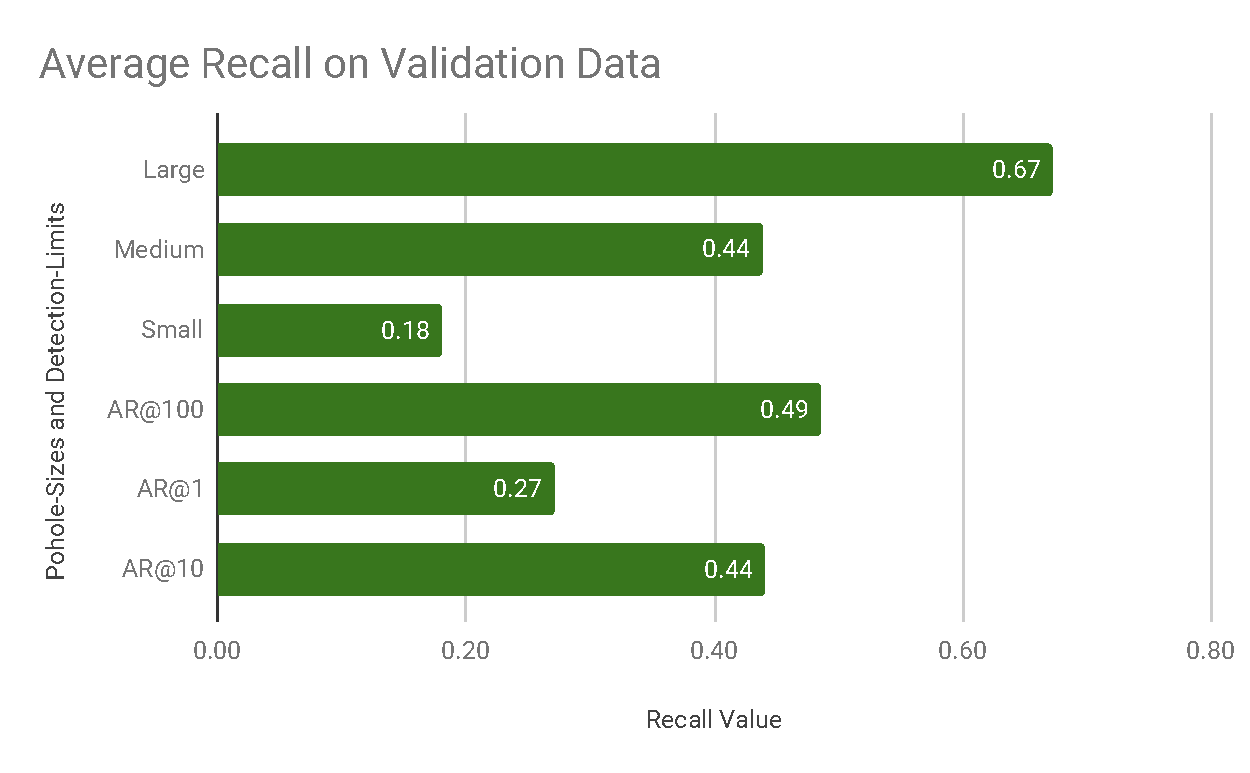
\includegraphics[width=\textwidth]{Average-Recall-on-Validation-Data}
                \caption{Validation-Recall Values (Compared)}
                \label{fig:recalls}
            \end{figure}
            
    \clearpage
    \section{Fall of Gradient Norm}
        The fall of gradient norm during training process is shown in Figure \ref{fig:gradient_norm}
        \begin{figure}[h]
            \centering
            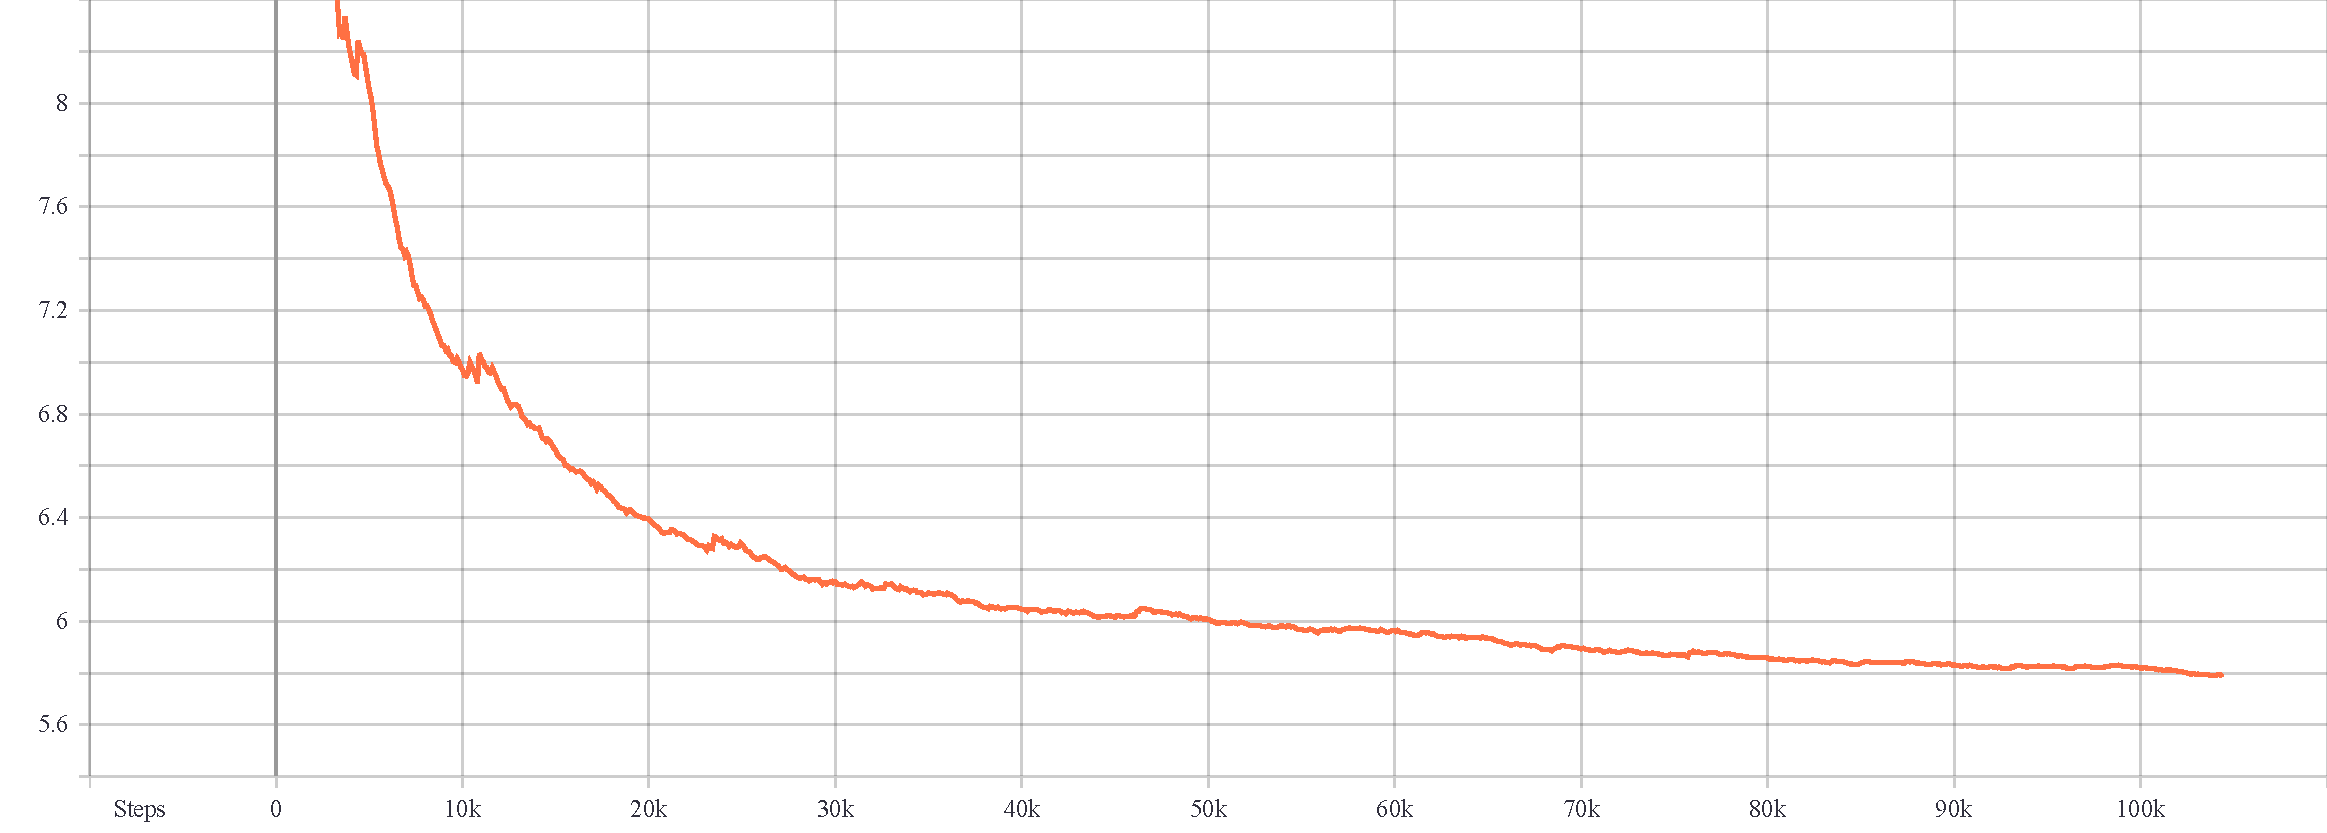
\includegraphics[width=\textwidth]{gradient-norm}
            \caption{Fall of Gradient-Norm During Training Process}
            \label{fig:gradient_norm}
        \end{figure}
        
    \section{Fall of Localization Loss}
        The fall of localization loss during training process is shown in Figure \ref{fig:loss_loc}
        \begin{figure}[h]
            \centering
            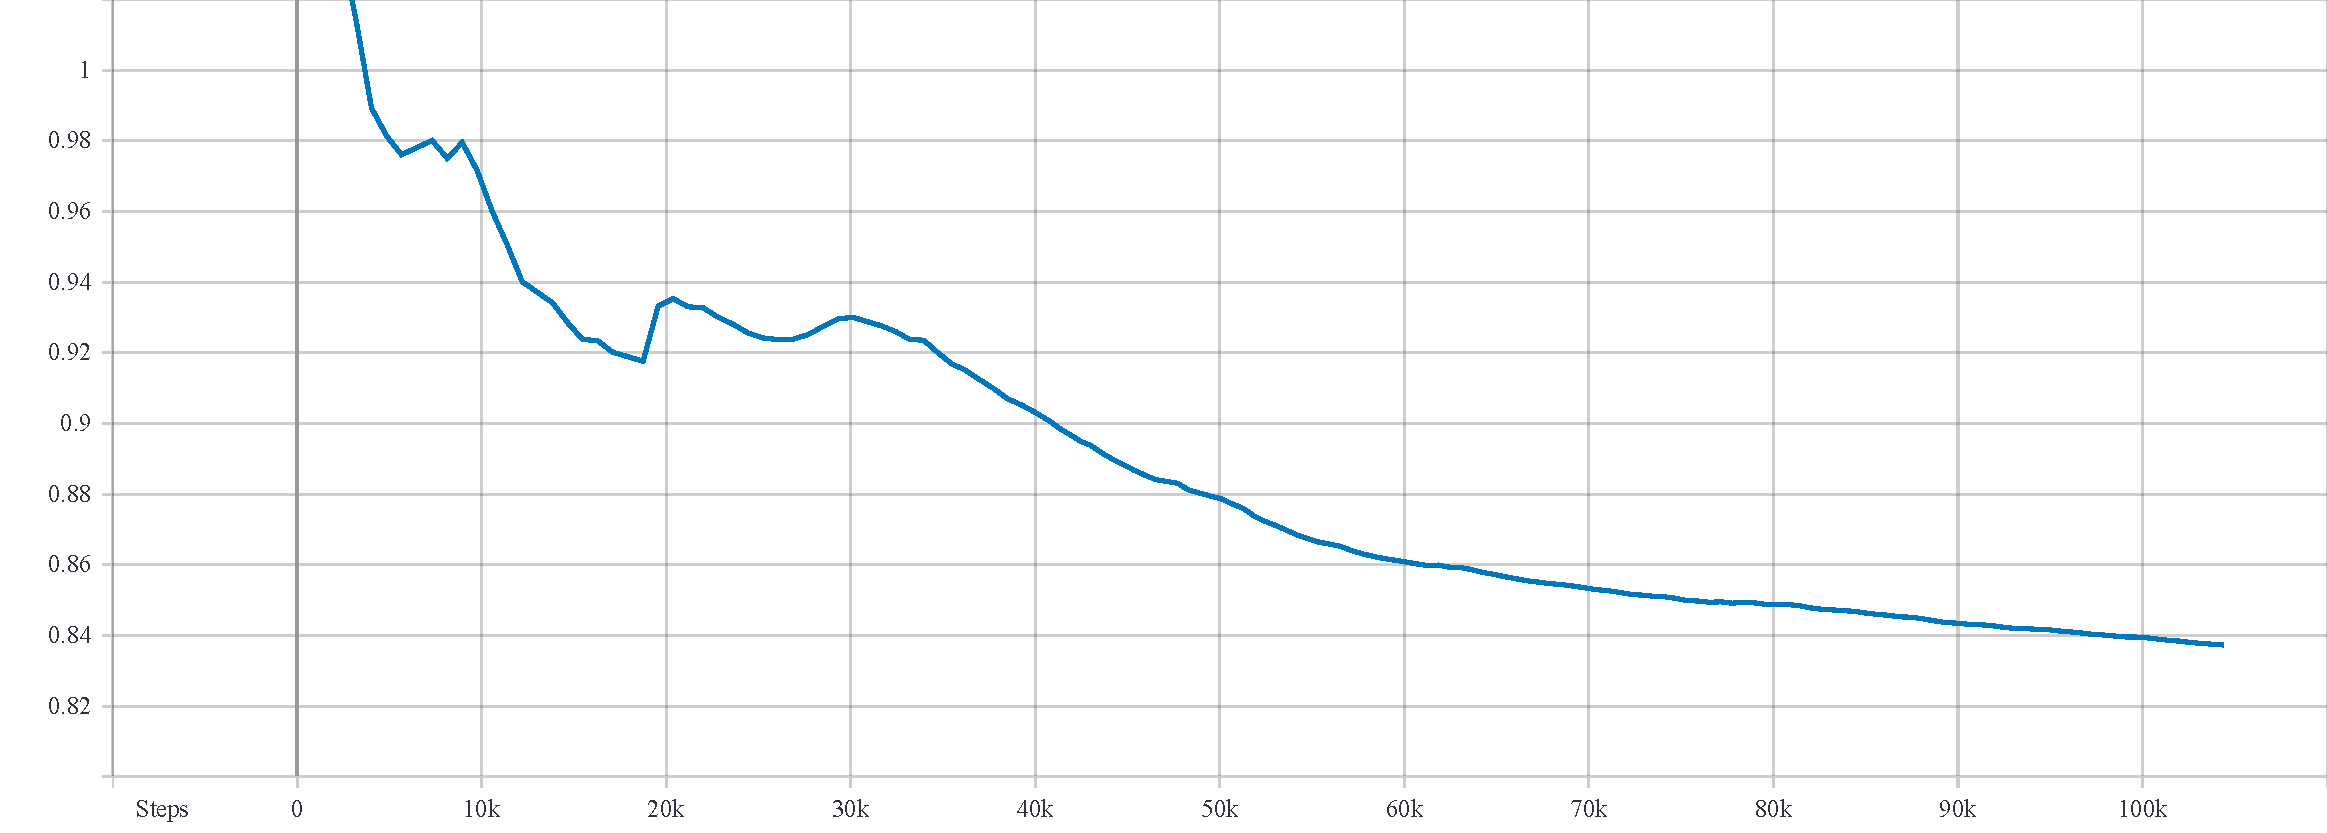
\includegraphics[width=\textwidth]{loss-localization}
            \caption{Fall of Localization-Loss During Training Process}
            \label{fig:loss_loc}
        \end{figure}
        
    \section{Fall of Regularization Loss}
        The fall of regularization loss during training process is shown in Figure \ref{fig:loss_reg}
        
        \begin{figure}[h]
            \centering
            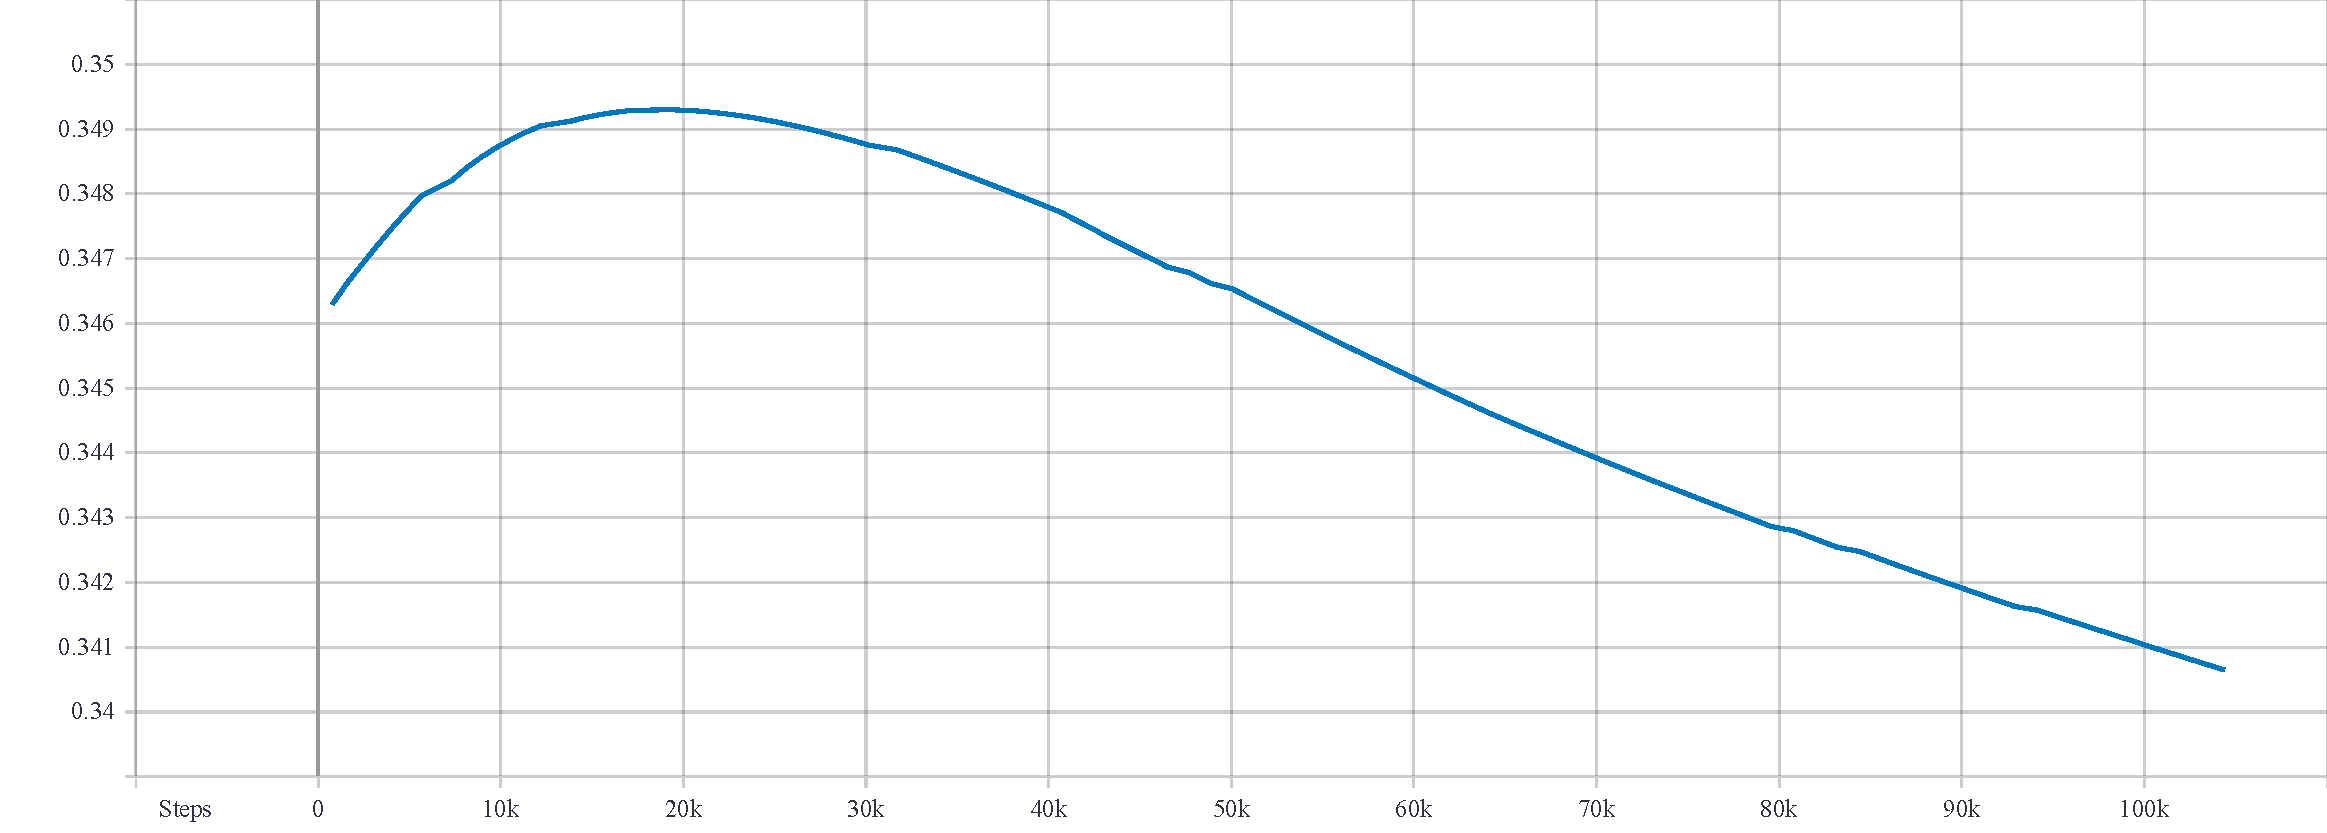
\includegraphics[width=\textwidth]{loss-regularization}
            \caption{Fall of Regularization-Loss During Training Process}
            \label{fig:loss_reg}
        \end{figure}
        
    \section{Changes of Learning-Rate}
        The decay of learning-rate during training process is shown in Figure \ref{fig:learning_rate}
        
        \begin{figure}[h]
            \centering
            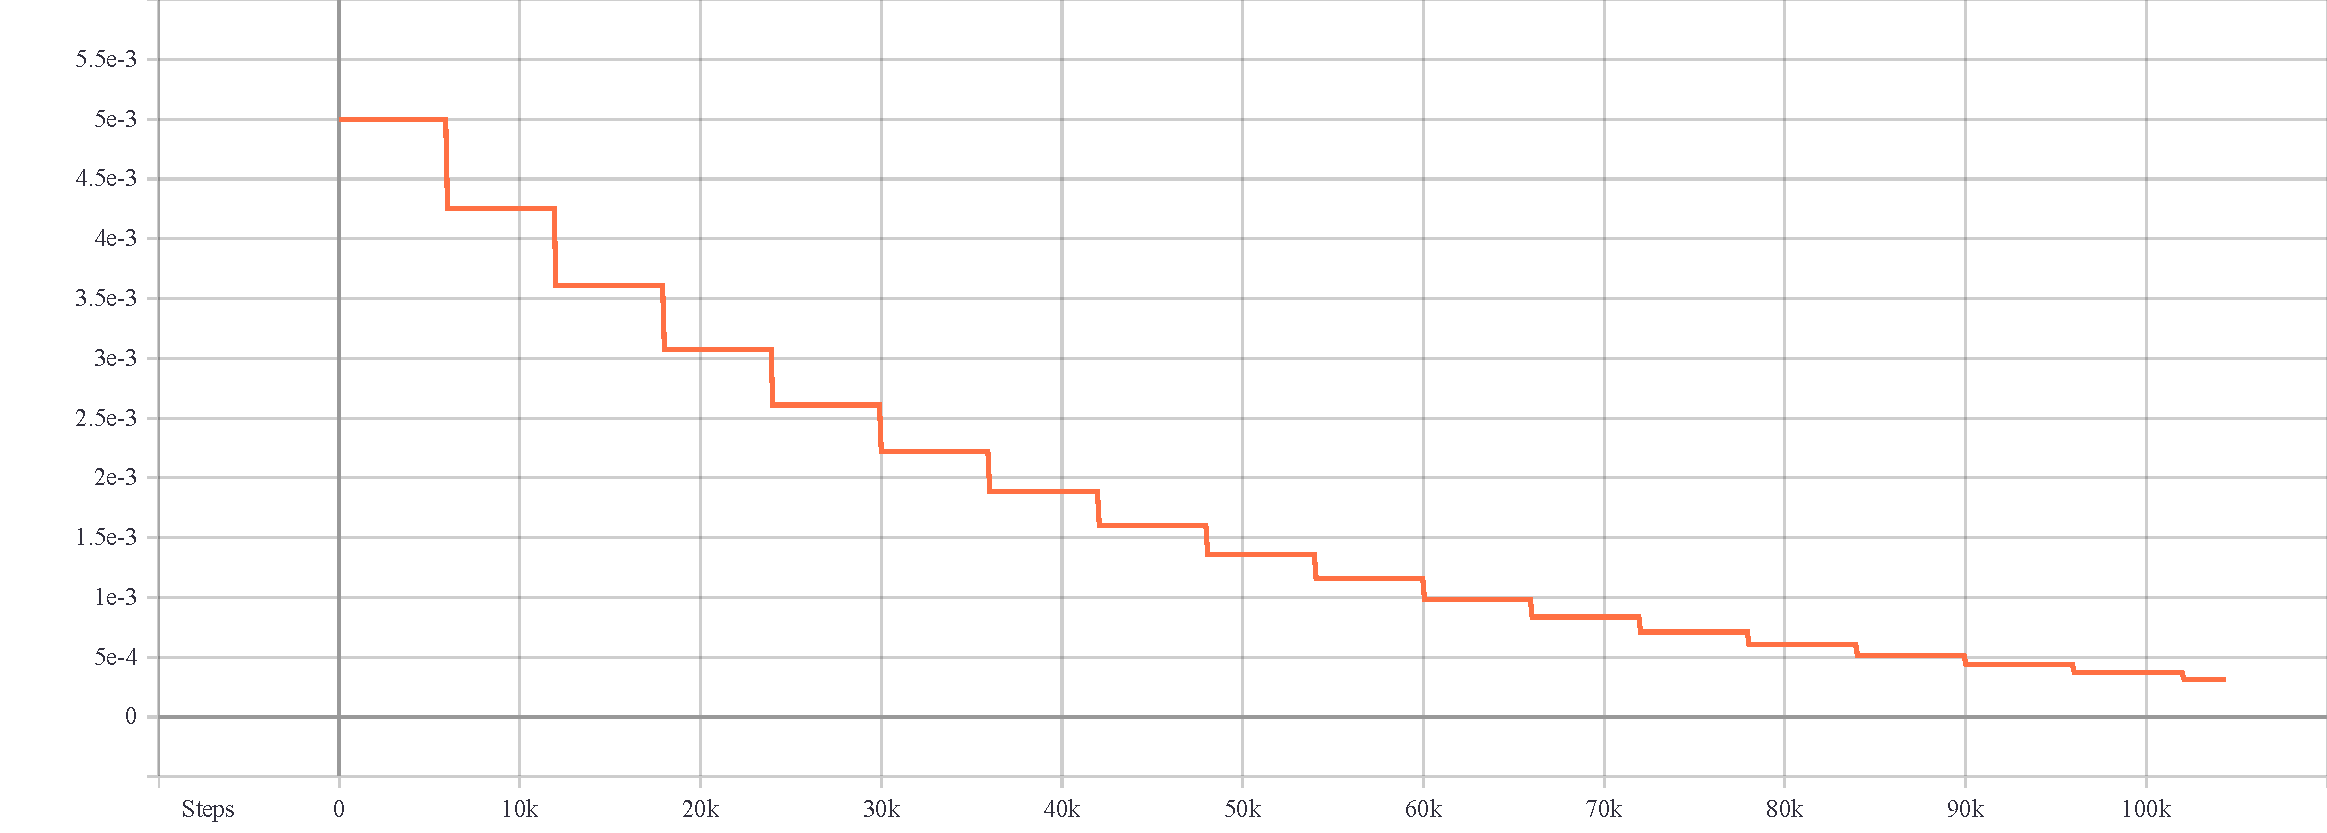
\includegraphics[width=\textwidth]{learning_rate}
            \caption{Decay of Learning-Rate During Training Process}
            \label{fig:learning_rate}
        \end{figure}
        
